\documentclass[11pt,a4paper]{article}

% ---------------------------------------------------------------------------
% Multi-Drone Cooperative Search with Random Faults — final report
% Single column, 11pt. Compile with pdflatex + bibtex (or latexmk -pdf).
% ---------------------------------------------------------------------------

\usepackage[utf8]{inputenc}
\usepackage[T1]{fontenc}
\usepackage[a4paper,top=2.2cm,bottom=2.2cm,left=2.45cm,right=2.45cm]{geometry}
\usepackage{lmodern}
\usepackage{microtype}

\usepackage{amsmath,amssymb}
\usepackage{graphicx}
\usepackage{tikz}
\usetikzlibrary{positioning,arrows.meta}
\usepackage{booktabs}
\usepackage{caption}
\usepackage{subcaption}
\usepackage{placeins}  % \FloatBarrier keeps figures within their subsection
\usepackage{xcolor}
\usepackage{enumitem}
\usepackage{csquotes}
\usepackage[numbers,square,sort&compress]{natbib}

\usepackage[hidelinks,colorlinks=true,linkcolor=black,citecolor=blue!50!black,urlcolor=blue!50!black]{hyperref}

% Document metadata: without these the PDF ships with an empty /Title and
% /Author, and viewers fall back to displaying the file name.
\hypersetup{
  pdftitle={Multi-Drone Cooperative Search with Random Faults},
  pdfauthor={Simone Rimondi},
  pdfsubject={Multi-Agent Systems project, MSc Artificial Intelligence, University of Bologna, A.Y. 2025/2026},
  pdfkeywords={multi-agent systems, deep reinforcement learning, Dueling Double DQN,
               parameter sharing, fault tolerance, partial observability, domain randomization}
}

% Figures live in report/figures/ (exported plots, diagrams, screenshots).
\graphicspath{{figures/}}

\captionsetup{font=footnotesize,labelfont=bf}

\setlength{\parskip}{0.08em}

% Convenience macros for recurring notation.
\newcommand{\gridsize}{32}
\newcommand{\rvis}{r_{\mathrm{vis}}}
\newcommand{\rcomm}{r_{\mathrm{comm}}}
\newcommand{\pfault}{p_{\mathrm{fault}}}
\newcommand{\nagents}{N}

\title{\textbf{Multi-Drone Cooperative Search\\ with Random Faults}\\[0.4em]
\large A fault-tolerant cooperative multi-agent system trained with\\ deep reinforcement learning, analysed through the multi-agent paradigm}

\author{Simone Rimondi\\[0.3em]
\small Student ID 0001189110\\[0.2em]
\small \href{mailto:simone.rimondi5@studio.unibo.it}{simone.rimondi5@studio.unibo.it}\\[0.3em]
\small Multi-Agent Systems\\
\small Master's Degree in Artificial Intelligence, University of Bologna\\
\small Academic Year 2025/2026}

\date{}

\begin{document}

\maketitle

\begin{abstract}
\noindent
We study cooperative target search by a team of drones on a partially
observable grid, under limited communication, a fixed time budget and~--- the
defining extension of this work~--- the possibility that any drone
permanently breaks at any moment, with no central authority to announce the
loss. A single Dueling Double DQN with parameter sharing drives every drone
from strictly per-drone inputs, batched into one forward pass only for speed;
per-episode domain randomization and a compact
context vector turn that one policy into a generalist across team size,
sensing, communication range, obstacle density, and fault rate. Fault
knowledge is fully decentralized: a wreck emits only a passive distress
beacon, and crash information spreads through the same range-limited map fusion
as any other observation, so each drone acts on a sound-but-possibly-stale
belief about how many teammates remain. We read the resulting system through
the multi-agent paradigm, namely coordination without protocols, environment-%
mediated (stigmergic) dispersion, an artefact and autonomy analysis, and an
epistemic account of fault handling, and we evaluate it empirically. The
single policy generalizes across every randomization axis, including
\emph{beyond} its trained ranges on team size, vision and communication; most
importantly, it degrades \emph{gracefully} under faults: across the
entire trained fault range success drops by under seven points while the team
loses, on average, close to half a drone, and even at more than triple the
trained fault rate it still completes nearly three missions in four, with no
cliff. We
close with an ethical and regulatory analysis (GDPR, the EU AI Act and its
military carve-out, and the autonomous-weapons scenario) that takes seriously
the dual-use nature of a capability whose fault tolerance would make an attack
swarm as resilient as a rescue one.
\end{abstract}

% Companion material. The tabular puts the three addresses in one column: the
% GitLab path alone is 79 characters, so set side by side they overrun the text
% block. Note that \url must be handed a literal URL, since it reads its
% argument verbatim and cannot be wrapped in a macro or a conditional.
\vspace{1.2em}
\begin{center}
\footnotesize
% Body font rather than typewriter, at footnotesize: the GitLab path is 79
% characters, and \url's default \ttfamily at \small overruns the text block by
% 65pt. Both settings are scoped to this group, so the bibliography's URLs keep
% their usual style.
\urlstyle{same}
\begin{tabular}{@{}r@{\hspace{1.1em}}l@{}}
\textbf{GitLab repository}  & \url{https://dvcs.apice.unibo.it/pika-lab/courses/ai-ethics/projects/rimondi2526-mas} \\[0.2em]
\textbf{GitHub repository}  & \url{https://github.com/simoswish02/Multi-Agent-Systems-Project} \\[0.2em]
\textbf{Trained weights}    & \url{https://huggingface.co/simoswish/MAS_MultiDroneExploration} \\[0.2em]
\textbf{Video walkthrough}  & \url{https://youtu.be/8dnRG6ZneP8}
\end{tabular}
\end{center}

\newpage

\tableofcontents

\newpage

\section{Introduction}
\label{sec:introduction}

When something must be found quickly over a large area --- a missing hiker,
survivors in a collapsed structure, the front of a spreading wildfire ---
teams of small autonomous aircraft are increasingly the tool of choice: they
are cheap, expendable, fast to deploy, and, above all, \emph{parallel}
\citep{queralta2020collaborative,julian2019distributed}. Yet the hard
problem in multi-drone search is not flight; it is coordination under
scarcity. Each vehicle perceives only a small neighbourhood of a large,
unknown environment; communication reaches only nearby teammates, so no
shared global picture exists; and the mission clock is unforgiving --- in
search and rescue, time \emph{is} the objective. A team that cannot divide
the search space effectively degenerates into an expensive single searcher.

This project adds to that already delicate setting the ingredient that
real operations always contain and idealized models usually omit:
\textbf{failure}. Small drones break --- motors fail, batteries die,
weather intervenes --- and they break \emph{mid-mission}, unpredictably,
without ceremony. A search system that presumes a fixed team is brittle in
exactly the situations that matter most. Worse, in a genuinely
decentralized setting a drone's death is not even \emph{announced}: its
teammates must discover the loss through their own sensing and
communication, and until they do, they coordinate with a phantom. Fault
tolerance in a multi-agent system is thus not one problem but three ---
surviving the loss (redundancy), learning of it (decentralized fault
knowledge), and adapting to it (re-planning the division of labour) --- and
this report treats all three as first-class design objects.

\paragraph{The problem.}
Concretely, we study the following task, formalized in
Section~\ref{sec:problem}. A team of $\nagents$ drones spawns co-located on
a corner of a $\gridsize\times\gridsize$ occupancy grid scattered with
obstacles; a single target, guaranteed reachable, is hidden at an unknown
cell. Each drone sees only a window of radius $\rvis$ around itself,
remembers what it has seen, and fuses its accumulated map with any teammate
within communication range $\rcomm$. The team has a hard budget of
$T_{\max}$ turns to physically reach the target. At every turn, any live
drone may irreversibly break with probability $\pfault$; a wreck stops
sensing, moving, and communicating, its turns still consume the budget, and
no one is notified --- fault knowledge spreads only through a passive
distress beacon and the ordinary map fusion. Success is binary and
team-level: \emph{some} drone reaches the target in time, or the episode
fails.

\paragraph{The approach.}
We solve the task with cooperative deep reinforcement learning under
parameter sharing \citep{gupta2017cooperative}: a single Dueling Double DQN
\citep{mnih2015human,vanhasselt2016double,wang2016dueling} drives every
drone, consuming that drone's private maps through a convolutional
architecture with an attention bottleneck, and trained on the pooled
experience of the whole team. Rather than fixing one operating condition,
every training episode randomizes the regime --- vision radius,
communication range, team size, obstacle density, and fault probability
\citep{tobin2017domain} --- and the sampled parameters that a real drone
could plausibly know are fed back to the network as a context vector,
together with two per-drone quantities: an identity (which breaks the
symmetry of parameter sharing and lets co-located drones adopt different
roles from the first step) and the drone's own \emph{belief} about how many
teammates remain operational. The result is a single generalist policy
that searches alone or in a team, myopic or far-sighted, in empty fields or
cluttered mazes --- and that experiences teammate death, and the need to
absorb it, as an ordinary feature of its world. The fault model demands
equal care on the learning side: a fault is exogenous bad luck, not a
consequence of behaviour, and Section~\ref{sec:training} shows why treating
it as anything but a truncation would silently bias the learned values.

\paragraph{Why this is a multi-agent systems study.}
A reinforcement-learning pipeline, however carefully engineered, is not by
itself the point of this report. The system is deliberately read, in
Section~\ref{sec:mas}, through the conceptual apparatus of multi-agent
systems \citep{wooldridge2009introduction,jennings2001agent}: the drones
are audited against the defining properties of agenthood; the environment
is analysed as a first-class abstraction that mediates and governs all
interaction; the map fusion is read as knowledge-level, protocol-free
communication over a distributed shared dataspace; the visited-cell traces
as a virtualized form of stigmergy; the fused map, the beacon, and the
action mask as coordination artefacts; the team's dispersion and post-fault
re-covering as emergent, self-organized structure that no component
specifies; and the whole design is placed on the autonomy spectrum ---
operationally autonomous, motivationally not. This analysis is not
decorative: it is what connects a concrete learned system to the questions
--- about coordination, openness, resilience, and responsibility --- that
the multi-agent perspective exists to ask. The same lens then carries the
final part of the report, where autonomy without deliberation and
competence without transparency become ethical and legal problems rather
than engineering trade-offs.

\paragraph{Contributions.}
The report makes the following contributions:

\begin{enumerate}[leftmargin=2em]
  \item \emph{A cooperative search environment with a decentralized fault
    model} (Sections~\ref{sec:problem}--\ref{sec:architecture}): a
    configurable grid world, built from scratch, in which drone failures
    are permanent, unannounced, and discoverable only through a distress
    beacon and range-limited map fusion --- no component ever accesses a
    global oracle of team state.
  \item \emph{A single generalist policy via domain randomization and
    context conditioning} (Sections~\ref{sec:architecture}
    and~\ref{sec:training}): one shared network that generalizes across
    team sizes, sensing and communication regimes, obstacle densities, and
    fault rates, with per-drone identity and believed-alive-count inputs
    enabling role differentiation and post-fault adaptation.
  \item \emph{A set of reinforcement-learning correctness decisions for
    fault-prone teams} (Section~\ref{subsec:train-correctness}): faults as
    bootstrapped truncations, retroactive team credit restricted to
    surviving drones, and shaping-robust checkpoint selection --- each with
    an explicit argument for why the obvious alternative is subtly wrong.
  \item \emph{A systematic multi-agent reading of the system}
    (Section~\ref{sec:mas}): a detailed mapping between the implemented
    mechanisms and the paradigm's core concepts --- agenthood, environment,
    coordination, artefacts, self-organisation, openness, autonomy, and
    multi-agent learning.
  \item \emph{An experimental protocol --- and, pending the conclusion of
    training, its results} (Section~\ref{sec:experiments}): seeded,
    reproducible evaluation of fault robustness, generalization across
    randomization axes, and the quantitative signatures of emergent
    coordination.
  \item \emph{A prospective ethical and regulatory analysis}
    (Section~\ref{sec:ethics}): the capability's dual-use profile, its
    treatment under the GDPR and the EU AI Act (including the military
    carve-out that exempts precisely the gravest use), an argument that
    the system as designed could not lawfully or ethically serve as an
    autonomous weapon, and a set of design commitments that follow.
\end{enumerate}

\paragraph{Roadmap.}
Section~\ref{sec:background} reviews the reinforcement-learning and
multi-agent-learning toolbox. Section~\ref{sec:problem} formalizes the task
as a partially observable, identical-interest Markov game with sequential
execution and defines the observation, communication, and fault models.
Section~\ref{sec:architecture} describes the implementation: environment,
observation encoding, neural architecture, and learning machinery.
Section~\ref{sec:training} covers the training methodology and its
correctness decisions. Section~\ref{sec:mas} develops the multi-agent
analysis at length. Section~\ref{sec:experiments} presents the experimental
design and results. Section~\ref{sec:ethics} develops the ethical and
regulatory analysis, and Section~\ref{sec:conclusions} concludes.
Appendices consolidate configuration details and reproduction instructions.

% TODO (figures pass): GUI teaser screenshot (4 drones, one wreck emitting
% a beacon) once final visuals are ready.

\section{Background}
\label{sec:background}

% Target length: ~5 pages. Self-contained toolbox; no project details here.
% Cite: sutton2018reinforcement, watkins1992qlearning, mnih2015human,
% vanhasselt2016double, wang2016dueling, hessel2018rainbow, littman1994markov,
% oliehoek2016concise, lowe2017multi, gupta2017cooperative,
% hernandezleal2019survey, tobin2017domain, peng2018sim.

\subsection{Sequential decision making}
\label{subsec:bg-mdp}
% TODO: MDP (S, A, P, R, gamma); policy, return, V/Q; Bellman optimality;
% Q-learning as off-policy TD control.

\subsection{Deep value-based reinforcement learning}
\label{subsec:bg-dqn}
% TODO: function approximation; DQN (experience replay + target network);
% overestimation bias and Double DQN; Dueling architecture Q = V + A - mean(A);
% n-step returns (bias/variance trade-off); truncation vs termination and why
% time-outs must bootstrap (used later in Sec. 5.4).

\subsection{Multi-agent reinforcement learning}
\label{subsec:bg-marl}
% TODO: Markov games generalizing MDPs; cooperative / competitive / mixed
% settings; core challenges: non-stationarity, scalability (joint action
% space), partial observability (Dec-POMDP flavour); solution spectrum:
% independent learners <-> joint-action learners <-> centralized training with
% decentralized execution (CTDE); parameter sharing as a practical middle
% ground; credit assignment in teams.

\subsection{Generalization and domain randomization}
\label{subsec:bg-dr}
% TODO: DR for robustness/transfer; context/task conditioning of a single
% policy (relation to goal-/context-conditioned RL).

% TODO: write draft.

\section{Problem Formulation}
\label{sec:problem}

This section formalizes the task that the rest of the report builds upon: a
team of drones must locate and reach a hidden target on a partially observable
grid, under limited communication, a fixed time budget, and the possibility
that any drone permanently breaks at any moment. We first describe the
scenario informally (Section~\ref{subsec:prob-scenario}), then cast it as a
partially observable Markov game with sequential execution
(Section~\ref{subsec:prob-model}), and detail its three defining ingredients:
the observation model (Section~\ref{subsec:prob-obs}), the communication
model (Section~\ref{subsec:prob-comm}), and the fault model
(Section~\ref{subsec:prob-fault}). Section~\ref{subsec:prob-objective} states
the objective and the reward function that operationalizes it.
Table~\ref{tab:notation} collects the notation used throughout the report.

\begin{table}[t]
\centering
\small
\begin{tabular}{llp{8.6cm}}
\toprule
\textbf{Symbol} & \textbf{Default} & \textbf{Meaning} \\
\midrule
$\mathcal{G}$ & $\{0,\dots,31\}^2$ & set of grid cells (fixed $\gridsize\times\gridsize$ map) \\
$\mathcal{O} \subset \mathcal{G}$, $\rho$ & $\rho \in [0.10, 0.30]$ & obstacle cells and obstacle density \\
$\mathcal{F} = \mathcal{G}\setminus\mathcal{O}$ & --- & free (traversable) cells \\
$g \in \mathcal{F}$ & --- & hidden target cell \\
$\nagents$, $i$ & $\nagents \in \{1,\dots,4\}$ & team size and drone index $i \in \{1,\dots,\nagents\}$ \\
$p_i^t \in \mathcal{F}$ & --- & position of drone $i$ at turn $t$ \\
$\mathcal{A}$ & $\{\mathrm{up},\mathrm{down},\mathrm{left},\mathrm{right}\}$ & action set (4 unit moves) \\
$\rvis$ & $\rvis \in \{1,\dots,6\}$ & vision radius (Chebyshev) \\
$V_i^t \subseteq \mathcal{G}$ & --- & vision set of drone $i$ at turn $t$ \\
$\rcomm$, $d_1$ & $\rcomm \in \{2,\dots,12\}$ & communication range and Manhattan distance \\
$\pfault$ & $\pfault \in [0, 0.003]$ & per-turn fault probability of a live drone \\
$\beta_i^t \in \{0,1\}$ & --- & alive flag of drone $i$ ($0$ = broken, permanent) \\
$K_i^t$ & --- & knowledge state (accumulated maps) of drone $i$ \\
$\mathcal{C}_i^t$, $\hat{n}_i^t$ & --- & crashed teammates \emph{known} to $i$; believed alive count \\
$T_{\max}$ & $200 \cdot \nagents$ & episode budget in agent-turns \\
$\gamma$ & $0.97$ & discount factor \\
\bottomrule
\end{tabular}
\caption{Notation used throughout the report. ``Default'' reports the value
or randomization range used in the final training configuration
(Section~\ref{sec:training}); parameters with a range are resampled at every
episode.}
\label{tab:notation}
\end{table}

\subsection{Scenario}
\label{subsec:prob-scenario}

The environment is an episodic grid world. At the beginning of every episode
a fresh $\gridsize\times\gridsize$ occupancy grid is generated: each cell is
independently declared an obstacle with probability $\rho$, and a single
target cell $g$ is placed uniformly at random among the free cells that are
reachable (under 4-connectivity) from the reference corner
$(0,0)$.\footnote{Reachability is verified with a breadth-first search at
generation time; layouts whose reachable region is empty are rejected and
resampled. The guarantee is stated with respect to the reference corner from
which the search is run.} A team of $\nagents$ drones spawns \emph{co-located}
on one randomly chosen corner of the map. The target position is unknown to
the drones; obstacles are likewise unknown until observed.

Each drone occupies one cell and, on its turn, moves to one of the four
axis-adjacent cells. Drones perceive only a local neighbourhood of their
position (Section~\ref{subsec:prob-obs}), accumulate what they have seen into
a private map, and can merge maps with teammates that are close enough
(Section~\ref{subsec:prob-comm}). The episode succeeds when any drone
\emph{physically reaches} the target cell --- merely spotting the target does
not end the episode, it only reveals its location to the observer (and, via
communication, to nearby teammates). The team operates under a hard budget of
$T_{\max}$ agent-turns; if the budget expires before the target is reached,
the episode fails.

Two features make the problem distinctly harder than classical cooperative
exploration. First, all drones start from the \emph{same} cell, so any
efficient division of the search space must be produced by the drones
themselves --- nothing in the environment assigns regions or roles. Second,
at any turn a live drone may irreversibly break with probability $\pfault$
(Section~\ref{subsec:prob-fault}); the survivors must absorb the loss and
re-cover the region the wreck leaves unsearched, without any central entity
telling them that a teammate is gone.

\subsection{Formal model}
\label{subsec:prob-model}

We model the task as a partially observable Markov game
\citep{littman1994markov,oliehoek2016concise} with identical-interest
(cooperative) structure and \emph{sequential execution},
\[
\mathcal{M} \;=\; \bigl\langle \mathcal{I},\; \mathcal{S},\;
\{\mathcal{A}_i\}_{i \in \mathcal{I}},\; T,\;
\{\mathcal{O}_i\}_{i \in \mathcal{I}},\;
\{r_i\}_{i \in \mathcal{I}},\; \gamma \bigr\rangle ,
\]
where $\mathcal{I} = \{1,\dots,\nagents\}$ is the set of drones and
$\mathcal{A}_i = \mathcal{A}$ for all $i$.

\paragraph{State.}
A global state
$s^t = \bigl(\mathcal{O},\, g,\, (p_i^t)_i,\, (\beta_i^t)_i,\,
(K_i^t)_i,\, t\bigr)$
collects the (episode-fixed) obstacle layout and target position, the drone
positions and alive flags, each drone's knowledge state, and the turn
counter. Including the knowledge states $K_i^t$ in $s^t$ is deliberate: the
per-drone observation is a deterministic rendering of $K_i^t$
(Section~\ref{subsec:prob-obs}), so the process is Markovian in $s^t$, and
partial observability arises precisely from the gap between $K_i^t$ and the
full state. Episode-level parameters
$\theta = (\rvis, \rcomm, \nagents, \rho, \pfault)$ are drawn at the start of
every episode and held fixed within it; their per-episode randomization is a
training-time design choice discussed in Section~\ref{sec:training}.

\paragraph{Sequential execution.}
Time advances in \emph{agent-turns}. At turn $t$ the acting drone is
$\iota(t) = \bigl((t-1) \bmod \nagents\bigr) + 1$, so a \emph{round} consists
of $\nagents$ consecutive turns in fixed order. Only the acting drone selects
an action; every other drone's position is unchanged. Crucially, a turn is
consumed \emph{even when the acting drone is broken}
(Section~\ref{subsec:prob-fault}): the clock never skips, so losing drones
never stretches the time budget. Sequential execution gives collisions and
map updates an unambiguous semantics (there are no simultaneous-move
conflicts to resolve) and matches the execution model of the learning
architecture, where all drones are driven by a single shared network
(Section~\ref{sec:architecture}).

\paragraph{Transition.}
The transition kernel $T$ composes a stochastic fault event with a
deterministic move. At the start of its turn, a live acting drone $i$ breaks
with probability $\pfault$ (its position freezes, $\beta_i \leftarrow 0$,
permanently). Otherwise it executes its action: the move succeeds if the
destination cell is inside the grid and not an obstacle, and the drone stays
in place if it is not. After moving, the drone's vision, the fault-beacon
detection, and the communication fusion update the knowledge states
(Sections~\ref{subsec:prob-obs}--\ref{subsec:prob-fault}). The only sources
of stochasticity are the episode initialization (layout, target, spawn
corner, $\theta$) and the fault process.

\paragraph{Action masking.}
The acting drone receives a binary mask over $\mathcal{A}$ that disables
moves leaving the grid or entering an obstacle in one of the four adjacent
cells. Because $\rvis \geq 1$, the adjacent cells are always inside the
drone's current vision set, so the mask adds no information beyond what the
drone has already observed --- it merely removes actions whose outcome
(bouncing in place) is already known, shrinking the exploration space. A
safety fallback re-enables all actions in the degenerate case where a drone
is boxed in on all four sides, guaranteeing the policy always has a legal
choice.

\paragraph{Episode end.}
The episode \emph{terminates} (success) as soon as the acting drone's new
position equals $g$. It is \emph{truncated} (failure) when $t$ exceeds
$T_{\max} = 200\cdot\nagents$, or early when all drones are broken, since no
state change is possible anymore. The distinction between termination and
truncation is not cosmetic: it changes the bootstrapping semantics of the
learning update, and Section~\ref{subsec:train-correctness} argues that
treating faults and time-outs as truncations is necessary for unbiased value
estimation.

\subsection{Observation model}
\label{subsec:prob-obs}

Each drone senses a square window centred on itself: at turn $t$, drone $i$'s
vision set is the Chebyshev ball
\[
V_i^t \;=\; \bigl\{\, c \in \mathcal{G} \;:\;
\lVert c - p_i^t \rVert_\infty \le \rvis \,\bigr\},
\]
i.e.\ a $(2\rvis{+}1)\times(2\rvis{+}1)$ box clipped to the grid. Sensing is
noiseless but strictly local: nothing outside $V_i^t$ is perceived.

What the policy consumes, however, is not the instantaneous percept but an
\emph{accumulated knowledge state}. Drone $i$ maintains
$K_i^t = (\mathit{Vis}_i, \mathit{Obs}_i, \mathit{Tgt}_i, \tau_i,
\mathit{Brk}_i, \mathcal{C}_i)$, a set of spatial maps over $\mathcal{G}$
updated after every move: for every cell $c \in V_i^t$,
\[
\mathit{Obs}_i(c) \leftarrow 1 \;\; \text{if } c \in \mathcal{O}, \qquad
\mathit{Tgt}_i(c) \leftarrow 1 \;\; \text{if } c = g, \qquad
\mathit{Vis}_i(c) \leftarrow 1 \;\; \text{otherwise}.
\]
All three maps are monotone --- knowledge is never forgotten, so a target
spotted once remains marked even after it leaves the field of view. The
trajectory map $\tau_i(c)$ counts how many times drone $i$ itself has
occupied cell $c$; unlike the other maps it is \emph{private}
(never communicated), acting as a personal revisit memory. The crash-site
map $\mathit{Brk}_i$ and the crashed-teammate set $\mathcal{C}_i$ record
fault knowledge and are described in Section~\ref{subsec:prob-fault}.

The observation $o_i^t \in \mathcal{O}_i$ delivered to the policy is a
deterministic, multi-channel rendering of $K_i^t$ plus the drone's own
position and the positions of \emph{live} teammates currently inside
$V_i^t$; its exact tensor encoding is an architectural matter deferred to
Section~\ref{subsec:arch-obs}. Conceptually, the accumulated maps play the
role of a hand-crafted belief state: they compress the interaction history
into a spatial summary, which is what allows a memoryless (non-recurrent)
policy to act reasonably in a partially observable world.

\subsection{Communication model}
\label{subsec:prob-comm}

Communication is proximity-bound, instantaneous, and content-fixed: what is
exchanged is \emph{world knowledge}, never commands or intentions. After
every turn, consider the communication graph over live drones with an edge
between $i$ and $j$ whenever their Manhattan distance satisfies
$d_1(p_i^t, p_j^t) \le \rcomm$. For every connected component $S$ of this
graph, the members merge their knowledge by an element-wise maximum,
\[
\mathit{Vis}_i \leftarrow \max_{j \in S} \mathit{Vis}_j, \qquad
\mathit{Obs}_i \leftarrow \max_{j \in S} \mathit{Obs}_j, \qquad
\mathit{Tgt}_i \leftarrow \max_{j \in S} \mathit{Tgt}_j, \qquad
\mathit{Brk}_i \leftarrow \max_{j \in S} \mathit{Brk}_j,
\]
together with the union of the crashed-teammate sets
$\mathcal{C}_i \leftarrow \bigcup_{j \in S} \mathcal{C}_j$, for every
$i \in S$. Merging over connected components makes communication
\emph{transitive} within a round: if $A$ is in range of $B$ and $B$ of $C$,
all three end up with identical fused maps even if $A$ and $C$ are far
apart --- intermediate drones act as relays.

Three properties of this mechanism are worth stressing, as they carry the
multi-agent analysis of Section~\ref{sec:mas}. First, fusion is
\emph{anonymous}: the max-merge keeps no record of who contributed which
cell, so shared knowledge detaches from its producer. Second, it is
\emph{persistent}: knowledge received in an encounter survives after the
drones part ways, because it is written into the receiver's own maps. Third,
it is \emph{selective}: the trajectory map $\tau_i$ is deliberately excluded
from fusion, so the revisit-avoidance signal remains individual. Wrecks
neither transmit nor receive --- a broken drone's maps freeze at fault time.

\subsection{Fault model}
\label{subsec:prob-fault}

The defining extension of this project is a random, permanent fault process.
At the start of its own turn, a live drone breaks with probability
$\pfault$, independently across drones and turns. The values used in
training are small per-turn probabilities with large episode-level effect:
at $\pfault = 0.003$ over $200$ rounds, a given drone breaks at some point
of the episode with probability $1 - 0.997^{200} \approx 0.45$.

A broken drone (a \emph{wreck}) is subject to the following semantics:

\begin{itemize}[leftmargin=1.5em]
  \item \textbf{Total incapacitation.} It no longer moves, senses, or
    communicates; its knowledge state freezes at fault time.
  \item \textbf{No time refund.} Its turns still occur and still consume the
    shared budget $T_{\max}$: the team loses capacity but gains no time.
  \item \textbf{Physically inert.} The crash cell is not an obstacle: live
    drones can traverse it, it never blocks a corridor (which preserves the
    reachability guarantee of the target), and the wreck is excluded from
    collision counting and from teammate-position observations.
\end{itemize}

\paragraph{Decentralized fault knowledge.}
No drone is notified of a teammate's fault. Instead, a wreck passively emits
a \emph{distress beacon}: a live drone $i$ discovers crash site $c_j$ of
drone $j$ when it either comes within communication range of it,
$d_1(p_i^t, c_j) \le \rcomm$, or sees it, $c_j \in V_i^t$. Upon detection,
$i$ records the crash in its own maps,
$\mathit{Brk}_i(c_j) \leftarrow 1$ and
$\mathcal{C}_i \leftarrow \mathcal{C}_i \cup \{j\}$, and this knowledge then
spreads through the ordinary map fusion of
Section~\ref{subsec:prob-comm} exactly like any other observation. Each
drone therefore holds a \emph{belief} about the team's size,
\[
\hat{n}_i^t \;=\; \nagents - \lvert \mathcal{C}_i^t \rvert ,
\]
which is sound but possibly stale: since $\mathcal{C}_i^t$ can only contain
drones that actually crashed, $\hat{n}_i^t$ never underestimates the true
alive count, but it may overestimate it for many rounds if the crash
happened far away. There is no global fault oracle anywhere in the system:
every quantity a drone acts upon --- including $\hat{n}_i^t$, which is fed
to the policy (Section~\ref{subsec:arch-context}) --- is derived from that
drone's own observations and from what teammates relayed to it. When the
last drone breaks, the episode is truncated early.

For learning purposes a fault is treated as a \emph{truncation} of the
broken drone's experience stream, not as a terminal state: the fault strikes
independently of the drone's state and action, and
Section~\ref{subsec:train-correctness} shows why conflating the two would
bias the learned values.

\begin{figure}[t]
\centering
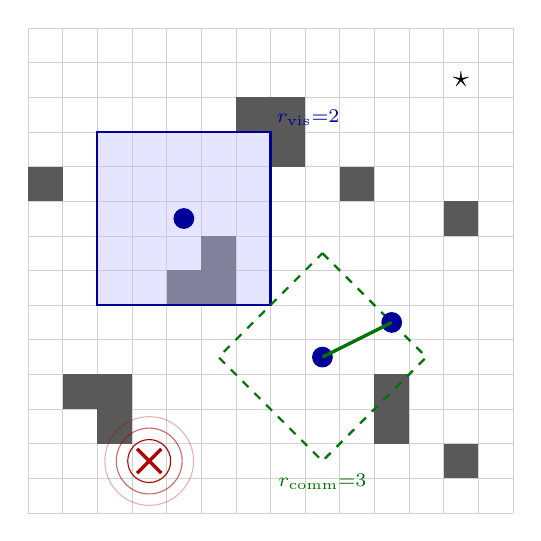
\begin{tikzpicture}[scale=0.44]
  % --- board ---
  \draw[step=1, gray!35, very thin] (0,0) grid (14,14);
  % --- obstacles ---
  \foreach \pos in {(1,3),(2,3),(2,2),(6,11),(7,11),(7,10),(10,2),(10,3),
                    (4,6),(5,6),(5,7),(12,8),(0,9),(9,9),(12,1)}
    \fill[black!65] \pos rectangle +(1,1);
  % --- hidden target ---
  \node at (12.5,12.5) {\large $\star$};
  % --- drone i: vision box (Chebyshev, r_vis = 2) ---
  \fill[blue!25, opacity=0.4] (2,6) rectangle (7,11);
  \draw[blue!60!black, thick] (2,6) rectangle (7,11);
  \fill[blue!60!black] (4.5,8.5) circle (0.30);
  \node[blue!60!black, anchor=south west] at (6.9,10.9) {\scriptsize $\rvis{=}2$};
  % --- drones j,k: comm range (Manhattan, r_comm = 3) ---
  \draw[green!45!black, thick, dashed] (8.5,7.5) -- (11.5,4.5) -- (8.5,1.5) -- (5.5,4.5) -- cycle;
  \fill[blue!60!black] (8.5,4.5) circle (0.30);
  \fill[blue!60!black] (10.5,5.5) circle (0.30);
  \draw[green!45!black, very thick] (8.5,4.5) -- (10.5,5.5);
  \node[green!45!black, anchor=north] at (8.5,1.4) {\scriptsize $\rcomm{=}3$};
  % --- wreck + distress beacon ---
  \draw[red!70!black, very thick] (3.15,1.15) -- (3.85,1.85);
  \draw[red!70!black, very thick] (3.15,1.85) -- (3.85,1.15);
  \draw[red!70!black] (3.5,1.5) circle (0.62);
  \draw[red!70!black, opacity=0.6] (3.5,1.5) circle (0.95);
  \draw[red!70!black, opacity=0.3] (3.5,1.5) circle (1.28);
\end{tikzpicture}
\caption{Schematic of the search scenario (illustrative $14\times14$ crop;
the actual map is $\gridsize\times\gridsize$). Dark cells are obstacles and
$\star$ is the hidden target. The left drone's square outline is its
Chebyshev vision window ($\rvis = 2$), inside which cells are revealed and
accumulated into its private map. The dashed diamond is the Manhattan
communication ball ($\rcomm = 3$) of the lower drone: the teammate inside it
fuses maps with it on every turn (solid link). The red cross is a wreck; its
concentric rings depict the distress beacon, which live drones detect when
they come within $\rcomm$ of the crash site (or see it), with no global
notification of the fault.}
\label{fig:scenario}
\end{figure}

\subsection{Objective and metrics}
\label{subsec:prob-objective}

The team's objective is to minimize the time at which the target is first
reached --- equivalently, to maximize the probability of reaching it within
the budget and, among successful strategies, to reach it as early as
possible. The task is identical-interest: no drone has a private goal, and
it is irrelevant \emph{which} drone reaches the target.

\begin{table}[t]
\centering
\small
\begin{tabular}{llll}
\toprule
\textbf{Term} & \textbf{Symbol} & \textbf{Value} & \textbf{Applied when} \\
\midrule
step penalty & $r_{\mathrm{step}}$ & $-0.3$ & every turn of a live drone (base cost of time) \\
wall penalty & $r_{\mathrm{wall}}$ & $-0.02$ & the move is invalid; the drone stays in place \\
revisit penalty & $r_{\mathrm{rev}} \cdot k$ & $-0.05 \cdot k$ & entering a cell drone $i$ already visited $k$ times \\
collision penalty & $r_{\mathrm{coll}} \cdot m$ & $-0.5 \cdot m$ & entering a cell occupied by $m$ other live drones \\
exploration bonus & $r_{\mathrm{expl}} \cdot c$ & $+0.02 \cdot c$ & $c$ cells newly added to the \emph{team's} discovered set \\
target reward & $R_{\mathrm{tgt}}$ & $+200$ & the drone's new cell is the target (terminates) \\
\bottomrule
\end{tabular}
\caption{Reward terms accumulated within a single turn of the acting drone
(values from the final configuration). Wrecks receive no reward: their turns
are no-ops.}
\label{tab:reward}
\end{table}

This objective is operationalized by the shaped per-turn reward of
Table~\ref{tab:reward}. On its turn, a live drone $i$ collects
\[
r_i^t \;=\; r_{\mathrm{step}}
\;+\; \mathbb{1}[\text{invalid move}]\, r_{\mathrm{wall}}
\;+\; \mathbb{1}[\text{valid move}] \bigl( k \, r_{\mathrm{rev}} + m \, r_{\mathrm{coll}} \bigr)
\;+\; c \, r_{\mathrm{expl}}
\;+\; \mathbb{1}[p_i^{t} = g]\, R_{\mathrm{tgt}} ,
\]
and the learning objective is the usual expected discounted return with
discount $\gamma$. Each term implements one facet of the task:

\begin{itemize}[leftmargin=1.5em]
  \item \emph{Time pressure.} The constant step penalty makes every turn
    costly, so faster target acquisition strictly dominates.
  \item \emph{Efficient coverage.} The exploration bonus counts cells that
    are new \emph{to the team} (the union of all discovered sets), not to
    the individual: re-discovering a region a teammate already swept earns
    nothing, which rewards complementary --- rather than duplicated ---
    search.
  \item \emph{Revisit avoidance.} The revisit penalty is linear in the
    drone's own prior visit count $k$ of the destination cell, so the
    cumulative cost of oscillating on the same spot grows quadratically with
    the number of passes; pacing back and forth is increasingly expensive.
  \item \emph{Dispersion.} The collision penalty charges co-location with
    live teammates. Since all drones spawn on the same corner, this is the
    only signal pushing the team to split; no region assignment or
    coordination protocol is provided (a point developed in
    Section~\ref{subsec:mas-coordination}).
  \item \emph{Team credit.} With the cooperative credit-assignment variant
    used in the final configuration (\texttt{shared\_target\_reward}), the
    terminal bonus $R_{\mathrm{tgt}}$ is granted to the whole surviving
    team rather than only to the finder, aligning individual returns with
    the identical-interest objective; drones that broke before the find are
    excluded. The learning-side implications of this choice are discussed in
    Section~\ref{subsec:train-correctness}.
\end{itemize}

At evaluation time (Section~\ref{sec:experiments}) the reward is set aside
and performance is reported through task-level metrics: \emph{success rate}
(fraction of episodes in which the target is reached within $T_{\max}$),
\emph{time-to-find} (turns elapsed at termination, over successful
episodes), \emph{coverage} (fraction of free cells discovered by the team),
and \emph{redundancy} (overlap between the regions swept by different
drones). The last two also serve as quantitative signatures of the emergent
division of labour analysed in Section~\ref{subsec:mas-emergence}.

% TODO (figures pass): consider adding a GUI screenshot next to the TikZ
% schematic once final visuals are ready.

\section{System Architecture}
\label{sec:architecture}

% Target length: ~7 pages. Keep faithful to docs/ARCHITECTURE.md (invariants!)
% and re-verify against code while drafting.
% Figures: module diagram (TikZ redraw of the mermaid graph); channel table;
% network architecture diagram; optional step_agent flowchart.

\subsection{Overview and module layout}
\label{subsec:arch-overview}
% TODO: entry points (main.py, eval_checkpoints.py), env/, agents/, training/,
% gui/, testing/; dependency diagram; config-driven design with
% configs/default.yaml as single source of truth.

\subsection{Environment implementation}
\label{subsec:arch-env}
% TODO: grid generation with BFS reachability guarantee; step_agent(i, a)
% internals (move/validate -> reward terms -> map update -> beacon detection ->
% communication fusion -> target check); action masking (4 move actions,
% invalid moves masked, boxed-in safety fallback); Gymnasium-compliant
% round-robin wrapper.

\subsection{Observation encoding}
\label{subsec:arch-obs}
% TODO: two streams — global (6 ch x 32^2: Visited, Obstacle, Trajectory,
% Target, Own_Position, Broken) and local (5 ch, cropped 13x13 patch, channel 4
% = Other_Position); channel semantics table; design choice: own position as a
% spatial channel (network recovers crop coordinates via argmax) instead of
% out-of-band coordinates; Broken channel = per-drone fault knowledge, feeding
% fault-awareness into the CNN spatially.

\subsection{Neural architecture}
\label{subsec:arch-network}
% TODO: GlobalMapCNN (ConvNeXt stages 96->192->384, FiLM after each stage,
% 8x8 token grid + CLS + ctx token -> 3-layer Transformer encoder; rationale:
% conv+attention hybrid restores global spatial-relational reasoning);
% LocalCNN (stride-1, dilated 7x7 depthwise, FiLM cross-conditioned on global
% features); dueling head Q = V + A - mean(A); LayerNorm/GRN only
% (batch-size-independent inference).

\subsection{Context vector}
\label{subsec:arch-context}
% TODO: CTX_DIM = 5: [vision, comm, n_agents, agent_id, n_alive_belief],
% normalized by domain-randomization maxima (build_ctx_norm); agent_id breaks
% parameter-sharing symmetry (identical spawn observations -> role
% differentiation at step 0); n_alive_belief enables re-planning as the
% believed team shrinks; rebuilt every round per drone; why obstacle_density
% and fault_prob are deliberately NOT context entries (observable from maps /
% unknowable in reality).

\subsection{Learning machinery}
\label{subsec:arch-learning}
% TODO: shared replay buffer; per-agent n-step windows; Double-DQN target,
% Huber loss, gradient clipping, hard target sync; batched greedy action
% selection (one forward pass for all live drones).

\subsection{Tooling and interaction modes}
\label{subsec:arch-tooling}
% TODO: GUI renderer (eval/play/simulate modes, fault slider, auto-nav toggle);
% BFS auto-nav override as an evaluation-only deterministic reference — never
% in training (invariant).

% TODO: write draft.

\section{Training Methodology}
\label{sec:training}

This section describes how the shared policy is actually trained: the
curriculum machinery that stages a run (Section~\ref{subsec:train-curriculum}),
the domain-randomization protocol (Section~\ref{subsec:train-dr}), the
exploration and learning-rate schedules (Section~\ref{subsec:train-schedules}),
a set of reinforcement-learning correctness decisions that the fault model
makes unusually delicate (Section~\ref{subsec:train-correctness}), and the
infrastructure that makes long runs reproducible and resumable
(Section~\ref{subsec:train-infra}).

\subsection{Curriculum}
\label{subsec:train-curriculum}

Training is organized as an ordered list of \emph{phases}, declared entirely
in the configuration file. Each phase specifies its episode count and may
override the team size, obstacle density, per-drone step budget, an
exploration reset, and --- crucially --- its own domain-randomization ranges;
anything not overridden falls back to the global settings. Two conventions
turn this list into a practical staging tool. First, \emph{a phase with zero
episodes is skipped}: alternative stagings are kept in the file and enabled
by editing a single number, so the exact shape of every run is versioned
alongside the code. Second, phase boundaries interact cleanly with resuming:
when a run restarts from a checkpoint, completed phases are skipped, the
active phase resumes from its saved episode index, and the phase's
exploration reset is suppressed (the checkpoint's annealed $\varepsilon$ is
kept rather than re-inflated).

The final run used in this report consists of a single main phase of
$50{,}000$ episodes with a per-drone budget of $200$ rounds and the full
randomization ranges of Table~\ref{tab:notation} active throughout ---
including the fault range --- preceded only by a zero-episode debug phase
kept for staging. Earlier exploratory stagings (shorter phases with narrower
ranges) informed the hyperparameters but do not contribute weights: the
reported policy is trained from scratch in the single phase. The curriculum
machinery is nevertheless part of the contribution: it is what made those
iterations cheap.

\subsection{Domain randomization}
\label{subsec:train-dr}

At the start of every episode the loop samples
$\theta = (\rvis, \rcomm, \nagents, \rho, \pfault)$ --- integers uniformly
(inclusive) and floats uniformly from their ranges --- applies it to the
environment via \texttt{set\_domain\_params}, and only then resets
(Section~\ref{subsec:arch-env}). The sampled ranges
(Table~\ref{tab:notation}) are wide by design. Vision spans myopic
($\rvis{=}1$: a $3\times3$ window) to far-sighted ($\rvis{=}6$); the
communication range spans nearly-isolated to easily-connected teams; the team
size spans a single drone --- where cooperation is moot and the policy must
search alone --- to four; obstacle density spans open fields to cluttered
mazes. The fault range $[0, 0.003]$ deserves its own reading: at the upper
end, a drone's probability of surviving all $200$ rounds is
$0.997^{200} \approx 0.55$, so the range spans ``faults never happen'' to
``losing roughly half the team over an episode is ordinary''. The policy is
therefore forced to be simultaneously a competent solo searcher, a
cooperative team member, and a survivor of team collapse --- with the
context vector (Section~\ref{subsec:arch-context}) telling it, at every
turn, which of these regimes it currently inhabits.

Per-episode resampling also acts as an implicit curriculum in expectation:
easy episodes (large vision, no faults, sparse obstacles) and hard ones
(blind, faulty, cluttered) interleave freely, which keeps a steady stream of
successful trajectories --- and hence of terminal reward signal --- flowing
into the replay buffer even before the policy masters the hard regimes.

\subsection{Schedules}
\label{subsec:train-schedules}

\paragraph{Exploration.}
$\varepsilon$-greedy exploration is annealed \emph{per episode} and
multiplicatively: starting from $\varepsilon_0 = 1$, each episode applies
$\varepsilon \leftarrow \max(0.05,\, 0.9995\,\varepsilon)$. The floor of
$0.05$ is reached after roughly $6{,}000$ episodes
($\approx 12\%$ of the run), after
which a residual $5\%$ of random actions keeps the buffer from collapsing
onto the greedy policy's own trajectory distribution. Exploration coins are
drawn per drone per turn (Section~\ref{subsec:arch-learning}), so within one
round some drones may explore while the others act greedily.

\paragraph{Learning rate.}
The learning rate follows a linear warmup ($10\%$ of the run,
$10^{-4} \to 5\times10^{-4}$) into a cosine annealing down to $10^{-6}$ at
the final episode. Two details are deliberate. The schedule is stepped
\emph{once per episode} rather than per gradient step: episode lengths vary
wildly across randomized regimes (a lucky find ends an episode in tens of
turns; a blind, faulty maze consumes the full budget), so stepping per
update would tie the schedule's shape to the difficulty mix rather than to
training progress. And it is sized by the \emph{total} episode count across
all phases, so the decay is a property of the run, not of any single phase.

\paragraph{Update cadence.}
One Double-DQN gradient step (Section~\ref{subsec:arch-learning}) runs every
$4$ agent-turns on minibatches of $16$ transitions from the shared replay
buffer; the target network is synchronized by hard copy every $500$ gradient
steps. Appendix~\ref{app:config} consolidates all values.

\subsection{Reinforcement-learning correctness decisions}
\label{subsec:train-correctness}

The fault model interacts with value-based learning in ways that are easy to
get silently wrong: nothing crashes, training even improves, but the learned
values answer a subtly different question than intended. This subsection
records the decisions taken, each with its rationale; together they
constitute the project's learning-side treatment of faults.

\paragraph{Time-outs bootstrap.}
Transitions record \emph{termination} only; running out of budget is a
truncation, and the final window still bootstraps the next-state value
(Section~\ref{subsec:bg-dqn}; \citealp{pardo2018time}). The time limit is an
experimental artifact --- the world does not end at turn $T_{\max}$ --- and
treating it as terminal would teach the network that states near the budget
boundary have no future, biasing values along every long trajectory.

\paragraph{A fault is a truncation, not a terminal.}
When a drone breaks, its pending $n$-step window is flushed immediately
\emph{with} bootstrapping ($\gamma^k$ for the $k$ steps accumulated), and no
further transitions are generated for it --- wrecks' no-op turns never enter
the buffer. The rationale mirrors the time-out case but is easier to get
wrong, because a fault \emph{feels} terminal for that drone. It is not, in
the sense that matters for learning: the fault strikes independently of the
drone's state and action ($\pfault$ is exogenous), so the states that
happened to precede a fault are not worth less than identical states that
did not. Zeroing the bootstrap would charge the value function for bad luck,
systematically depressing the values of \emph{whatever the drone happened to
be doing} when it broke --- noise injected as signal, growing with
$\pfault$. Bootstrapping instead treats the fault as censoring: the return
is simply observed no further. The alternative --- modelling faults
\emph{inside} the value function by scaling values by survival probability
--- would require the network to know $\pfault$, which is exactly the
quantity Section~\ref{subsec:arch-context} argues a deployed drone cannot
know.

\paragraph{Team credit is retroactive, and only for the living.}
With the shared terminal reward enabled
(Section~\ref{subsec:prob-objective}), the finder's terminal reward arrives
through the environment, while every \emph{other} live drone's bonus is
written retroactively into its most recent still-pending window, which is
then marked terminal. This mechanism has two consequences worth making
explicit. It requires $n \geq 2$: with one-step windows every transition is
emitted immediately, and there is nothing pending to credit (the
configuration is validated at run start). And it excludes drones that broke
before the find --- their windows were flushed at fault time, so their
experience of the episode ends, correctly, with what they themselves
observed: a drone that died exploring an empty quadrant should not learn
that dying there is worth the team's eventual success.

\paragraph{Selection is protected from shaping drift.}
Every $1{,}000$ episodes the current policy is evaluated near-greedily
($\varepsilon = 0.05$) on a \emph{fixed} set of $20$ instances: the
randomization draw and the map layout are both derived deterministically
from fixed seeds, and one seed reproduces layout and fault sequence alike
(Section~\ref{subsec:arch-env}), so successive evaluations differ only in
the policy. The checkpoint-selection rule is success-dominant: a new best
requires a strictly higher success rate, with mean reward used as a
tie-breaker only at $100\%$ success. This shields model selection from the
shaped reward terms of Table~\ref{tab:reward} --- a policy must not be
preferred because it harvests exploration bonuses more efficiently while
finding the target less often.

\paragraph{No planner contamination.}
The BFS auto-navigation override of Section~\ref{subsec:arch-tooling} never
runs during training --- neither in the episode loop nor in the in-training
evaluation that selects checkpoints. In the loop it would corrupt the data
distribution (transitions would reflect the planner's policy, not the
network's); in the selection it would corrupt the metric (checkpoints would
be ranked partly on the planner's competence). It exists strictly as an
analysis instrument for Section~\ref{sec:experiments}.

\subsection{Infrastructure and reproducibility}
\label{subsec:train-infra}

Training runs on a SLURM-managed HPC cluster (single GPU per run), launched
by a batch script that stages temporary files on node-local scratch storage;
the identical entry point runs unchanged on a workstation, which is how
short debugging stagings were iterated. Full runs log per-episode scalars to
TensorBoard --- reward, length, success, the sampled randomization values,
the number of drones lost to faults, $\varepsilon$ and the learning rate ---
so a run's difficulty mix and its learning progress can be inspected jointly.

\paragraph{Checkpointing and resumption.}
Three kinds of checkpoint are written: \texttt{best.pt} (weights only, on
every new evaluation best), periodic per-phase snapshots, and
\texttt{last.pt}, which additionally carries the full training state ---
optimizer, learning-rate schedule position, $\varepsilon$, gradient-step
counter, and curriculum position (phase and episode index). Resuming from
\texttt{last.pt} therefore continues the run \emph{as if uninterrupted},
with one deliberate exception: the replay buffer is not serialized (at
$2\times10^5$ full observation pairs it would dwarf the weights), so a
resumed run refills its buffer from fresh experience. A separate
weights-only warm-start mode initializes a brand-new run (fresh optimizer,
schedules, and curriculum) from an existing policy. On checkpoint
compatibility: the observation layout and context dimensionality changed
when the fault model was introduced (new Broken channel, new belief entry),
so weights from the pre-fault ancestor of this project are architecturally
incompatible --- training for this report starts from scratch.

\paragraph{Parallel checkpoint evaluation.}
Because the in-training evaluation is intentionally small (20 instances), a
separate \emph{watcher} process --- spawned automatically at run start ---
evaluates every periodic checkpoint on $200$ randomized-but-seeded episodes
as soon as it is written, appending to an incremental, crash-safe summary
and producing a final ranking when training ends. This offloads thorough
evaluation from the training loop (which would otherwise stall for minutes
every $1{,}000$ episodes) and, in practice, provides a second opinion on
checkpoint selection at no wall-clock cost to training.

% Figure TODO (after the final run): training curves — episode reward,
% eval success rate, epsilon/LR schedules, n_broken histogram.

\section{The System Through the Multi-Agent Paradigm}
\label{sec:mas}

The preceding sections described \emph{what} was built and \emph{how} it is
trained. This section changes register and asks what kind of system it is.
Multi-agent systems are not merely a technology but an engineering perspective:
a way of decomposing a problem into autonomous, interacting, situated components
and of locating where a system's intelligence actually resides
\citep{jennings2001agent,wooldridge2009introduction}. Read through that lens the
drone team instantiates a remarkably wide slice of the multi-agent conceptual
apparatus, from agenthood and the environment-as-abstraction through
coordination, artefacts, self-organization, resilience and graduated autonomy to
multi-agent learning. Throughout, every conceptual claim is anchored to a
concrete mechanism from Sections~\ref{sec:problem}--\ref{sec:training}, and the
section closes by asking, honestly, what a richer multi-agent design would add
and at what cost.

\subsection{Why a multi-agent formulation}
\label{subsec:mas-why}

It is worth beginning with the question the rest of the section presupposes: why
is this a multi-agent system at all, rather than one program steering four
vehicles? The answer is that the defining constraints of the task, not
implementation taste, rule the centralized alternative out along the three
dimensions that classically motivate the agent paradigm: distribution, autonomy
and interaction \citep{jennings2001agent,zambonelli2003signs}.

\emph{Distribution of sensing and knowledge.} No component of the system ever
holds the global state. Each drone perceives a Chebyshev window of radius
$\rvis$ and knows, beyond that, only what it has accumulated or been told. A
central controller would need the union of all observations at every turn, but
the communication model is range-limited: drones farther apart than $\rcomm$
cannot exchange anything. Centralized control over a communication-limited team
is not merely inefficient; during the frequent, deliberate intervals in which the
team is partitioned into disconnected communication components, it is
\emph{physically unimplementable}. The problem itself is distributed, so the
control must be.

\emph{Autonomy as a fault-tolerance requirement.} The fault model sharpens the
argument to its most concrete form. A centralized controller is a single point of
failure, and this project's central premise is that components \emph{do} fail, at
random, mid-mission. If the deciding entity resided in one drone and that drone
broke, the team would be decapitated. In the actual design, every drone carries
the full decision-making apparatus, its own copy of the shared policy, and the
death of any subset of drones leaves every survivor as capable as before.
Autonomy here is not an aesthetic commitment: it is what makes graceful
degradation possible at all.

\emph{Interaction as the source of system-level competence.} Finally, the task
is one no single drone solves well: a lone searcher covers area linearly in time,
while a well-dispersed team covers it in parallel. The system-level competence,
sweeping the map quickly, avoiding duplicated effort and re-covering the sectors
of fallen teammates, is located in no individual policy evaluation; it arises
\emph{between} the drones, from their interactions through fusion, mutual
observation and shared spatial traces. That is precisely what distinguishes a
multi-agent system from a parallel implementation of a single-agent one
\citep{wooldridge2009introduction}.

One clarification prevents a recurring misunderstanding: the drones share network
\emph{weights}, and weight sharing is a training-time device, not a runtime
coupling. At execution each drone evaluates its own copy of the function on its
own inputs; no activation, gradient or decision crosses drone boundaries. Four
copies of the same brain, fed four different experiences, are four agents, just
as identical twins are two people.

\subsection{Drones as agents}
\label{subsec:mas-agents}

``Agent'' is a contested term, but a broadly shared core defines it as a
computational system situated in an environment and capable of autonomous action
in pursuit of its design objectives, with the \emph{weak notion of agency}
requiring autonomy, reactivity, proactiveness and social ability
\citep{wooldridge1995intelligent,franklin1996agent}. This subsection audits the
drone against each requirement, and is equally explicit about which stronger
notions the drone does \emph{not} satisfy.

\paragraph{Autonomy: encapsulated control.}
The most fundamental computational reading of autonomy is encapsulation of
control: an agent is a locus of decision that cannot be \emph{invoked}, other
components being able to influence it only through data, never by calling its
behaviour as one calls a procedure \citep{wooldridge1995intelligent}. The drones
satisfy this literally. Nothing in the system commands a drone: teammates cannot
move it, interrupt it or query it, and the only thing that ever crosses the
boundary between two drones is world knowledge, through fusion. Each turn
consists of reading \emph{its own} observation and context, evaluating \emph{its
own} policy copy, and acting. Even the round-robin scheduling does not breach
encapsulation: it serializes \emph{when} drones act, a property of the
environment's clock, not \emph{what} they decide.

\paragraph{Situatedness.}
Agents act \emph{in} and \emph{through} an environment, and their action cannot
be divorced from the context in which it occurs \citep{suchman1987plans}. The
drone's entire interface to the world is environmental: it perceives by revealing
cells around its position, acts by moving to adjacent cells, and even its
communication is situated, fusion being triggered by spatial proximity rather
than by addressing a recipient. There is no action-at-a-distance anywhere in the
system, and the policy's inputs are spatial through and through: position, fault
knowledge and history all reach the network as \emph{maps}, an architectural echo
of the fact that for this agent context is location.

\paragraph{Reactivity, with state.}
The classical formalization of a non-trivially reactive agent equips it with
internal state: a perception function from environment states to percepts, a
state-update function folding each percept into an internal state, and an action
function from internal states to actions \citep{wooldridge2009introduction}. The
drone realizes the triple exactly: perception is the vision update (cells within
$V_i^t$, plus beacon detection); the state update is the monotone accumulation
into $K_i^t$, merged with teammates' contributions by fusion; the action function
is the Q-network's masked greedy selection over the rendering of $K_i^t$. That
internal state is what lifts the drone above a thermostat-style pure reflex: two
drones on the same cell with the same vision act differently if their
\emph{histories} differ, because their maps do.

\paragraph{Proactiveness: distilled, not represented.}
Agents are expected to exhibit goal-directed behaviour, taking initiative rather
than merely responding to stimuli \citep{wooldridge1995intelligent}. The drone is
unambiguously goal-directed in behaviour, since it systematically expands
coverage, avoids re-searching and homes in on the target once its location enters
the map, yet nowhere in the drone does the goal \emph{exist as an object}. There
is no symbol denoting ``find the target'', no explicit desire, no plan. The
goal-directedness was distilled at training time from the reward function of
Table~\ref{tab:reward} into the value estimates that now drive action selection.
In the classical dichotomy, the drone is \emph{goal-oriented} rather than
\emph{goal-governed}: its objective is implicit in the structure of its behaviour
rather than explicitly represented and reasoned over. This is a genuine
trade-off, not a defect, and Section~\ref{subsec:mas-beyond} discusses what
explicit goals would buy, and cost.

\paragraph{Social ability.}
The drone's social repertoire is narrow but real: it donates its accumulated
knowledge to whoever comes within $\rcomm$, incorporates teammates' knowledge
symmetrically, perceives nearby live teammates through the Other\_Position
channel, and both emits, passively as a wreck, and consumes distress information.
The next subsection analyses why this thin, language-free interaction layer is
nonetheless a coordination mechanism of some sophistication.

\paragraph{What the drone is not.}
Against the \emph{strong} notion of agency, with mental states, beliefs and
intentions in the technical sense of belief--desire--intention architectures
\citep{rao1995bdi,bratman1987intention}, the drone plainly falls short, and it is
worth being precise about where. The per-drone knowledge state is
belief-\emph{like}: private, partial, possibly stale, updated by observation and
testimony. But it is a fixed-schema spatial data structure, not a revisable base
of propositions; the drone cannot represent ``teammate 2 probably went north'',
let alone reason about what teammate 2 believes. Deliberation, in the sense of
weighing candidate intentions, is likewise absent, replaced by a single amortized
function evaluation. The system thus occupies a definite point in the agent
design space: fully agentive in the weak sense, deliberately sub-cognitive in the
strong one.

\subsection{The environment as a first-class abstraction}
\label{subsec:mas-environment}

A recurring lesson of multi-agent engineering is that the environment is not
scaffolding around the agents but a design dimension in its own right: an active
entity with its own state, dynamics and rules, through which agents perceive, act
and interact \citep{weyns2007environment}. This project embodies that stance
structurally: \texttt{DroneSearchEnv} is not a thin arena but the locus of most of
the system's semantics. The agent package is larger in absolute size, but almost
all of it is network definition and learning machinery; the world model,
including every rule of interaction, lives entirely on the environment side.
Four environmental
responsibilities deserve explicit notice. \emph{Topology and locality}: the grid,
its Chebyshev vision neighbourhoods and its Manhattan communication distances
define what ``near'' means, and thereby delimit perception, interaction and
fusion; locality is not a property agents happen to have but a rule the
environment enforces uniformly on everyone. \emph{Dynamics}: the fault process
lives in the environment, not in the agents, since drones do not decide to fail,
the world fails them, and the same holds for the episode clock, including the
rule that wrecks' turns still consume budget. \emph{Mediation}: every interaction
between drones, whether fusion, mutual sighting or beacon detection, is computed
by the environment as a side effect of spatial configuration, so drones have no
channel to each other that bypasses the world, which is exactly the
situated-interaction discipline \citet{weyns2007environment} argue for. And
\emph{governance}: the action mask constrains the space of legal behaviour at its
source, while the reward terms of Table~\ref{tab:reward} are environmental
legislation, the incentive structure under which autonomous behaviour is shaped
without ever being commanded.

The methodological payoff appeared already in Section~\ref{sec:architecture}:
because the environment owns the rules, the agents could be swapped (random,
keyboard-driven, BFS-guided, learned) with zero change to the world's semantics,
which is what lets Section~\ref{sec:experiments} run the learned policy and the
BFS auto-navigation override over identical seeded instances.

\subsection{Interaction and coordination}
\label{subsec:mas-coordination}

Coordination, in the sense of managing the interdependencies between concurrent
activities so that a collection of agents behaves as a coherent ensemble, is the
central problem any multi-agent system must solve. This system solves it with a
combination that is instructive precisely because of what it lacks: there are no
messages, no protocols, no negotiation, no roles assigned by any authority.
Coordination arises from three mutually reinforcing mechanisms.

\paragraph{(a) Knowledge-level communication without a language.}
When two drones fuse maps, what travels is world knowledge (``these cells are
free, these are obstacles, the target is here, teammate 3 crashed there'') and
nothing else: no requests, commands, commitments, or any of the performatives
that agent communication languages provide \citep{finin1994kqml}. The omission is
principled rather than lazy. Speech acts exist to coordinate \emph{deliberating}
agents: a request makes sense when the receiver can decide whether to honour it.
Between sub-cognitive policies there is no deliberation to address, and the task
is identical-interest, so there is nothing to negotiate over. What remains
genuinely useful to exchange is exactly what \emph{is} exchanged: factual
knowledge, whose fusion is monotone (element-wise maximum) and therefore
order-independent, idempotent and conflict-free. The design question ``what
should agents say to each other?'' is answered here with ``nothing; they should
compare notes''.

\paragraph{(b) The fused map as a shared dataspace.}
The resulting pattern has the character of a \emph{blackboard} or generative
dataspace rather than of message passing
\citep{nii1986blackboard,gelernter1985generative}: the three properties of
generative communication, namely that emitted information outlives its producer,
is accessible by content rather than by address, and decouples interacting
parties in time and identity, all hold of the fused knowledge. A cell discovered
by drone 1 at round 10 shapes drone 4's decision at round 150, long after the
encounter that transmitted it, possibly via a relay chain (1 fused with 2, later
2 with 4) such that 1 and 4 were \emph{never} within range of each other; and
because fusion is an anonymous maximum, knowledge carries no provenance, the
receiver acting on ``the target is at $(r,c)$'' identically whether it saw the
target itself or inherited the fact third-hand. The team's effective medium of
coordination is thus a distributed, eventually-consistent shared map, differing
from a classical blackboard in having no central board: every drone carries its
own replica, and proximity events are the synchronization protocol.

\paragraph{(c) Stigmergic traces, virtualized.}
The third mechanism is coordination through the \emph{traces} of activity, the
pattern Grass\'e named stigmergy: work performed modifies the environment, and
the modified environment directs subsequent work
\citep{grasse1959reconstruction,parunak1997go}. The Visited and Trajectory
channels are precisely such traces. A drone's movement writes a growing mark into
the shared knowledge (visited cells, own visit counts); those marks then
\emph{repel} future search, economically via the revisit penalty and the
nullified exploration bonus, behaviourally via whatever avoidance the trained
policy has internalized, steering drones away from consumed regions exactly as an
evaporating pheromone steers ants away from depleted paths, with the sign
inverted: repulsion, not attraction. One twist distinguishes this from textbook
stigmergy. The traces are not written into the physical grid, the world's cells
having no memory of visits, but into the drones' \emph{shared beliefs},
propagating through fusion rather than sitting at a location. It is stigmergy
over a distributed cognitive medium rather than over matter; the coordination
logic (work marks the field; marks direct work) is identical.

\paragraph{Learned conventions instead of designed protocols.}
What binds these mechanisms into actual coherence, namely \emph{who} goes where
and \emph{how} the team splits, is not specified anywhere. It is a convention
learned by co-training. During training, all drones' experience flows into one
network; behaviours that reduce duplicated coverage were systematically
reinforced by the team's shared exposure to the collision penalty, the
team-novelty exploration bonus and the shared terminal reward. The identity input
of Section~\ref{subsec:arch-context} gives the convention something to condition
on: from the very first round, when all drones stand on the same cell with
identical maps, the policy can map \emph{different identities to different
headings}, realizing an implicit division of the map without any sector ever
being represented, assigned or agreed upon. This is coordination knowledge stored
in weights rather than in protocol state, with consequences, adaptivity and
opacity in equal measure, that Sections~\ref{subsec:mas-beyond}
and~\ref{subsec:eth-responsibility} examine.

\subsection{An artefact perspective}
\label{subsec:mas-artefacts}

The agents-and-artefacts view of multi-agent systems holds that a MAS is
populated not only by agents but by \emph{artefacts}: non-autonomous,
function-oriented computational entities that agents use, which mediate their
activities, and in which designers can embed coordination machinery
\citep{omicini2008artifacts}. Artefacts do not pursue goals; they provide
operations, behave predictably, and serve. The distinction is illuminating here
because it cleanly separates the system's two kinds of components, and locates
several load-bearing pieces of the design on the artefact side of the line.

The clearest instance is the \emph{accumulated map}: a cognitive artefact with a
definite function (aggregate spatial knowledge), a usage interface (written by
moving and sensing, read at every decision as the network's input) and entirely
reactive, predictable dynamics (monotone accumulation and max-merge; it never
acts on its own). It mediates agent--environment interaction, since the drone
acts on the world \emph{as represented by its map}, and through fusion
agent--agent interaction as well: the fused map is a coordination artefact in
exactly the sense in which tuple spaces and blackboards are
\citep{gelernter1985generative,omicini2008artifacts}. The same reading covers the
\emph{distress beacon}, since a wreck is, in death, reduced to an artefact that
manifests one fact to whoever passes, and the \emph{action mask}, a constraining
artefact that does not decide for the agent but delimits its option space,
artefacts enabling and constraining in the same gesture.

Two observations sharpen the picture. Artefacts are where the \emph{designer's}
intelligence lives at runtime: the policy is learned and opaque, while the map
semantics, the fusion rule, the mask and the reward machinery are designed and
transparent; and the system's verifiable properties (fusion never loses
knowledge, masks never permit illegal moves, wrecks never block corridors) are
all artefact properties, inspectable and predictable by construction
\citep{omicini2008artifacts}. And the tooling of
Section~\ref{subsec:arch-tooling} extends the taxonomy to the humans in the loop:
the GUI, the TensorBoard scalars and the seeded evaluation harness are
observation artefacts through which the \emph{engineer} perceives the MAS, the
instrumentation layer that makes an otherwise opaque adaptive system engineerable
at all.

\subsection{Self-organization and emergence}
\label{subsec:mas-emergence}

Self-organization denotes the acquisition of structure by a system through
internal, distributed processes, without external control
\citep{ashby1962principles,camazine2001self}; emergence denotes the appearance of
coherent macro-level patterns not reducible to, nor explicitly encoded in, the
components' individual specifications \citep{goldstein1999emergence}. Both terms
apply to this system, but sloppily applied they explain nothing; the value lies
in stating precisely \emph{what} is designed and \emph{what} emerges.

\emph{Designed} are the local rules: the reward terms a drone experiences (all
computable from its own transition), the fusion rule, the fault process and the
training procedure itself. \emph{Not designed}, that is nowhere represented in
code or in weights as an explicit specification, are the team-level regularities
the trained system is expected to exhibit: the early-episode radial dispersion
from the shared spawn corner; the partition of the map into implicit,
identity-correlated search sectors; the complementarity of coverage, meaning low
overlap between drones' swept regions; and the re-absorption of a dead drone's
sector by its survivors. Each of these is a macro-pattern over the joint
trajectory of the team, produced by four independent evaluations of one function
that has never been trained on, or even given access to, any team-level
objective, each drone's inputs remaining strictly local throughout.

The classical checklist for self-organized coordination
\citep{camazine2001self}, namely multiple interacting units, local information
only, no external director, positive and negative feedback, is met, with the
mechanisms identifiable one by one: negative feedback is the repulsion from
consumed regions (revisit penalty, spent exploration bonus, collision penalty)
that spreads the team out; positive feedback is the attraction created when the
target's location enters the shared map and propagates through fusion, collapsing
the team's search into a pursuit. The balance of the two is exactly what the
policy has had to learn.

Two honest qualifications distinguish this from natural self-organization. First,
the organization is \emph{trained into} the system: the attractors of the
collective dynamics were shaped by fifty thousand episodes of gradient descent
against a designer-chosen reward, which is self-organization at execution time
and teleology at training time. Second, these team-level regularities have the
status of \emph{design intent with partial quantitative support}: of the three
signatures defined as their empirical test,
Section~\ref{subsec:exp-qualitative} delivers coverage complementarity and leaves
the two trajectory-level ones (dispersion over time, post-fault re-covering
latency) to future instrumentation.

\subsection{Fault tolerance, openness, and resilience}
\label{subsec:mas-resilience}

Multi-agent systems are routinely credited with robustness through redundancy and
decentralization; this project turns that slogan into a concrete, testable
mechanism. Three layers of the design implement it.

\paragraph{Structural redundancy.}
Every drone is a complete, interchangeable searcher: same policy, same sensing
model, same authority (none over the others). The task requires \emph{some} drone
to reach the target, not any particular one, so no individual's loss is
qualitatively worse than another's; combined with the environment-level
guarantees that wrecks neither block corridors nor cost reachability, any single
survivor retains in principle the ability to complete the mission alone, degraded
in time but not in kind. This is the redundancy-based robustness familiar from
biological collectives \citep{camazine2001self}, engineered deliberately.

\paragraph{A weak form of openness.}
The team's composition changes at runtime: an episode that begins with four
agents may end with one. In multi-agent terms the system is \emph{semi-open}:
departures occur unannounced, but no agent ever joins. Even this weak openness
has real consequences. Nothing in any drone's machinery assumes a fixed team size
(the policy is conditioned on team size and believed alive count, and per-agent
structures are allocated per episode), and no drone's correct functioning depends
on any other drone existing. The design would extend to arrivals, the context and
fusion machinery being indifferent to \emph{which} drones exist, though the
trained policy has never experienced them: a gap between the architecture's
openness and the policy's that is easily conflated.

\paragraph{Epistemic decentralization: acting on belief, not knowledge.}
The most distinctive layer is informational. No drone is told the team's true
state: each maintains $\mathcal{C}_i^t$, the crashed teammates it knows of, and
acts on the belief $\hat n_i^t = \nagents - |\mathcal{C}_i^t|$. This is a
genuine, if minimal, epistemic structure: a private, first-order factual belief
state, updated by two canonically distinct sources, direct observation (entering
beacon range or sight of a crash) and testimony (fusion with a better-informed
teammate), with the propagation dynamics of a gossip process, fault knowledge
spreading through the chance encounters of the communication graph at a rate
governed by $\rcomm$ and by how the policy moves the drones. The soundness
property established earlier, that $\hat n_i$ never undercounts the living, has a
behavioural face: a drone's error is always in the direction of
\emph{overestimating} its team, continuing to rely, for a while, on a searcher
that no longer exists. The interval between a fault and a given survivor's
discovery of it is thus the system's window of miscoordination, and its cost is
an empirical question that Section~\ref{subsec:exp-faults} takes up. The design
decision worth defending here is the refusal of the tempting alternative, a
global fault oracle broadcasting team state, which would be simpler and would
quietly reintroduce exactly the centralized, distance-insensitive information
channel whose absence defines the problem.

Note finally how the three layers compose: redundancy makes survivors
\emph{sufficient}, epistemic decentralization makes them eventually \emph{aware},
and context conditioning makes them \emph{adaptive}, since $\hat n_i$ feeds the
policy, so discovering a death is not merely bookkeeping but an input that
licenses recalibrating the division of labour. Fault tolerance is not a module in
this system; it is a property of the composition.

\subsection{The autonomy spectrum}
\label{subsec:mas-autonomy}

Autonomy is graduated, not binary, a lesson institutionalized in the level
taxonomies of applied domains, from driving automation's six levels
\citep{sae2021j3016} to the human-delegation hierarchies of military doctrine
\citep{dod2012autonomy}. Placing this system honestly on that spectrum matters
twice: once for conceptual hygiene, and once because the placement determines
which ethical questions Section~\ref{sec:ethics} must answer.

The distinction that organizes the spectrum is between \emph{automatic} systems,
executing pre-specified stimulus-response rules however elaborate, and
\emph{autonomous} ones, which select and adapt their own courses of action toward
a goal under conditions their designers did not enumerate. The drones sit
unambiguously on the autonomous side: no trajectory, sweep pattern or contingency
table exists anywhere in the system, the mapping from situations to actions was
learned, and it adapts online to circumstances (team size, sensing regime,
obstacle layout, teammate deaths) that vary per episode and per turn. The BFS
auto-navigation override is the clarifying foil: \emph{that} is an automatic
component, a fixed and verifiable procedure, and Section~\ref{sec:experiments}
uses it precisely because its behaviour, unlike the policy's, is fully
explainable.

Yet the drones' autonomy is strictly \emph{executive and operational}, not
motivational. They choose their actions; they do not choose, weigh, reformulate
or abandon their goal, which was fixed by the designers, half at design time in
the reward function and half at training time in its distillation into values,
with no runtime process able to revise it. In delegation terms
\citep{dod2012autonomy}: the human specifies \emph{what} (find the target) and
every constraint on \emph{how} (the reward's economy of time, collision and
coverage); the system autonomously resolves everything below that line and
nothing above it. Two boundary facts make the point concrete. The drones cannot
refuse the mission or trade it off against anything, there being nothing else in
their value system; and the capability that looks most like initiative,
re-planning the division of labour when the team shrinks, is itself
goal-subordinate adaptation triggered by a belief update, in service of the same
fixed objective.

This placement, with high operational autonomy, zero motivational autonomy, no
runtime human in the loop and an opaque learned decision function, is exactly the
profile for which accountability questions are sharpest: the system's behaviour
is neither predictable enough to certify like an automatic device, nor deliberate
enough to interrogate like a reasoning agent. Section~\ref{sec:ethics} takes up
precisely this configuration.

\subsection{Learning in the multi-agent system}
\label{subsec:mas-learning}

Parameter sharing \citep{gupta2017cooperative} places this design at a specific
point of the CTDE continuum \citep{kraemer2016multi,lowe2017multi}: training-time
centralization consists \emph{only} of pooling experience into one replay buffer
and one set of weights, with no centralized critic, no access to teammates'
observations or actions, and no global state anywhere in the loss. Every
transition that trains the network is something some individual drone actually
experienced, and execution is correspondingly clean, since the batched action
selection is a wall-clock optimization with no informational content. The
deployment artefact is a fully decentralized policy in the strictest sense. The
same choice disposes of two MARL classics at once: the \emph{symmetry} of a
shared policy at a shared spawn is broken by the identity entry of the context
vector, and \emph{scalability} follows from never materializing the joint
anything, since sequential execution plus per-drone argmax means the joint action
space whose exponential growth motivates much of the literature simply never
appears, team size entering as a conditioning scalar rather than a
dimensionality. What sharing does \emph{not} remove is the moving-target problem,
each drone's optimal behaviour still depending on teammates' evolving behaviour,
and here the design accepts the standard empirical wager of parameter-shared
MARL: that co-evolution of one policy converges more gracefully than co-evolution
of $\nagents$.

\paragraph{The platform as a multi-agent laboratory.}
A final identity shift is worth recording: the same artefact that trains the
policy is, unchanged, an agent-based simulation platform
\citep{bonabeau2002agent}, a micro-level model whose macro-behaviour is studied
by controlled manipulation. The seeded, parameterized evaluation harness is
methodologically identical to a simulation experiment design: hold the population
of instances fixed, vary one factor ($\pfault$, $\rcomm$, team size), and measure
macro-level responses. In this reading Section~\ref{sec:experiments} is an
agent-based ``what-if'' study of the trained collective: what happens to a
searching society as its members become mortal.

\subsection{What a richer multi-agent design would add}
\label{subsec:mas-beyond}

The system's multi-agent machinery is deliberately minimal, and the analysis
above should not read as a claim that minimal is optimal. It is worth stating
what each classical layer this design omits would offer, and what it would cost,
both as intellectual honesty and as a roadmap.

\emph{Explicit communication protocols} \citep{finin1994kqml} would let drones
exchange intentions rather than facts (``I will sweep the north-east quadrant''),
enabling explicit task allocation and with it verifiable non-overlap guarantees
instead of statistically-learned dispersion. The cost is the machinery this
design conspicuously avoids: message semantics, conversation state, commitment
handling, and the robustness of all of it to the death of either partner
mid-protocol, a non-trivial concern in precisely this problem.

\emph{Deliberative architectures} \citep{rao1995bdi} would make goals and plans
explicit and inspectable. The gain is not primarily performance but
\emph{explainability}: a belief--desire--intention drone answers ``why did you go
north?'' with an intention trace, where the present drone can answer only with a
Q-value, a difference whose ethical weight
Section~\ref{subsec:eth-responsibility} makes precise. The cost is the classical
one: hand-authored plan libraries in a domain whose main difficulty is exactly
what resists concise symbolic specification.

\emph{Organizational structure}, meaning roles, formations and an explicit
division of the map, would replace learned conventions with designed ones,
gaining predictability and losing the seamless re-adaptation that makes the fault
response work: a role structure must be re-formed when its occupants die, whereas
the learned convention degrades continuously with $\hat n_i$.

\emph{Programmable coordination media}
\citep{gelernter1985generative,omicini2001tuple} offer perhaps the most natural
upgrade path, since the system already has a coordination medium (the fused map)
with a fixed policy (max-merge). Making that medium programmable, with a fusion
rule that could age knowledge, prioritize target and crash information under
bandwidth limits, or maintain provenance, would relocate coordination
intelligence from the opaque policy into an inspectable artefact, the move the
artefact literature explicitly recommends \citep{omicini2008artifacts}.

The common thread is a single trade-off, and it is the honest summary of this
section: every engineered layer buys transparency, verifiability and designer
control, and pays in brittleness and specification burden; the learned-minimal
design buys adaptivity across regimes that would each demand their own
specification, and pays in opacity. This project sits knowingly at the learned
end. The experimental section measures what that position buys; the ethical
section confronts what it costs.

\section{Experimental Evaluation}
\label{sec:experiments}
\draftpending

% Target length: ~8 pages. BLOCKED until trained weights are available.
% Strategy: write captions and narrative structure NOW, drop in numbers and
% figures once the final checkpoint is evaluated.
% Tooling already in place: eval_checkpoints.py, testing/evaluate_policy.py
% (--axis fault and other OFAT axes, --seeds, --auto-nav).

\subsection{Experimental setup}
\label{subsec:exp-setup}
\draftpending
% TODO: checkpoint under test (best.pt of the final curriculum); fixed seed
% sets; episodes per configuration (~200-500); hardware; metrics: success
% rate, time-to-find (steps over successful episodes), coverage %, redundant
% visit ratio / overlap, per-drone contribution; confidence intervals via
% seed repetition.

\subsection{Baselines}
\label{subsec:exp-baselines}
\draftpending
% TODO: random policy; BFS auto-nav (deterministic sweep reference — NOT an
% upper bound, discuss why); optionally single drone vs team (value of
% cooperation).

\subsection{Generalization across randomization axes}
\label{subsec:exp-generalization}
\draftpending
% TODO: OFAT sweeps via testing/evaluate_policy.py — vision radius, comm
% range, team size, obstacle density; one curve per axis; in-range vs
% out-of-range probes.

\subsection{Fault robustness}
\label{subsec:exp-faults}
\draftpending
% TODO (headline experiment): success/time vs fault_prob (including p=0
% reference); behavioural adaptation: trajectories before/after a teammate's
% crash; does a survivor re-cover the dead drone's sector?; effect of comm
% range on how fast fault knowledge spreads (belief lag vs performance).

\subsection{Ablations}
\label{subsec:exp-ablations}
\draftpending
% TODO (time permitting): no communication (comm range 0); context without
% n_alive_belief; shared vs individual terminal reward.

\subsection{Qualitative analysis}
\label{subsec:exp-qualitative}
\draftpending
% TODO: trajectory plots, visit heatmaps, dispersion snapshots; link back to
% Sec. 6.6 emergent signatures (coverage-overlap measurements).

\subsection{Discussion and limitations}
\label{subsec:exp-discussion}
\draftpending
% TODO: simulation-only; grid abstraction; i.i.d. fault model; no adversary;
% sim-to-real gap.

% TODO: run experiments once weights are ready, then draft.

\section{Ethical and Regulatory Analysis}
\label{sec:ethics}

A grid-world simulation processes no personal data, harms no one, and needs
no licence. The analysis of this section is therefore explicitly
\emph{prospective}: it asks what would follow --- ethically and legally ---
if the capability this project prototypes were embodied in real aircraft
over real terrain. The exercise is not hypothetical hand-wringing. The task
specification of Section~\ref{sec:problem} --- find a hidden target in
minimum time, under partial observability, with a team resilient to
attrition --- is the abstract core of application profiles that range from
the unambiguously beneficial to the gravest imaginable, and the technical
analysis of Section~\ref{sec:mas} (in particular the autonomy placement of
Section~\ref{subsec:mas-autonomy} and the opacity trade-off of
Section~\ref{subsec:mas-beyond}) supplies exactly the vocabulary the
ethical questions are posed in. We proceed from the dual-use diagnosis
(Section~\ref{subsec:eth-dualuse}), through the two European regulatory
frameworks that would govern civilian deployments --- data protection
(Section~\ref{subsec:eth-gdpr}) and the AI Act
(Section~\ref{subsec:eth-aiact}) --- to the military scenario that escapes
both (Section~\ref{subsec:eth-laws}), the responsibility problem that
underlies all of it (Section~\ref{subsec:eth-responsibility}), and a set of
concrete design commitments (Section~\ref{subsec:eth-recommendations}).

\subsection{A dual-use capability}
\label{subsec:eth-dualuse}

Nothing in this system knows what its target \emph{is}. The environment
marks one cell; the policy learns to reach it quickly. Instantiate the
target as a missing hiker and the system is a search-and-rescue asset
\citep{queralta2020collaborative}; as a wildfire front, an environmental
monitor \citep{julian2019distributed}; as a person of interest, a
surveillance tool; as a military objective whose localization triggers
engagement, a component of a weapon system. The capability is
deployment-agnostic by construction --- and that is the precise sense in
which it is \emph{dual-use}: the same artifact serves civilian and military
ends without modification, the classification hinging entirely on context
of use.

Two features of this particular design sharpen the point beyond the generic
observation that search generalizes. First, the project's central technical
contribution --- fault tolerance through redundancy, decentralized fault
knowledge, and graceful degradation (Section~\ref{subsec:mas-resilience})
--- is exactly the property that makes a hostile swarm hard to defeat:
resilience to random attrition and resilience to defensive fire are the
same competence under different descriptions. Second, the single-policy
generalization across team sizes, sensing ranges, and communication regimes
(Section~\ref{subsec:train-dr}) is, read adversarially, robustness of the
threat across countermeasure conditions. One cannot celebrate these
properties in Section~\ref{sec:mas} and disown them here; the designer of a
capability owns its profile of uses, and the honest response is not denial
but analysis --- which uses are governed by what rules, where the rules run
out, and what the designer can do unilaterally
(Section~\ref{subsec:eth-recommendations}).

\subsection{Data protection: the GDPR lens}
\label{subsec:eth-gdpr}

Consider first the benign deployment: drones searching for missing persons
or assessing disaster zones over inhabited areas. Real perception is not an
oracle bit but cameras and sensors over public and private space, and
aerial imagery of identifiable individuals is personal data; its processing
falls squarely under the General Data Protection Regulation
\citep{gdpr2016} --- or, when the operator is a law-enforcement authority
acting in that capacity, under its sibling instrument for police
processing, Directive (EU) 2016/680. Four consequences of the GDPR's
architecture bear directly on a drone-search deployment.

\emph{Lawful basis and purpose limitation.} Consent is structurally
unavailable --- one cannot consent whoever happens to be under the flight
path --- so processing must rest on another Article~6 basis: protection of
vital interests fits the rescue scenario, public task fits civil
protection. The decisive discipline is purpose limitation: data collected
to find a missing person may not drift into general surveillance of
whoever else was observed --- \emph{mission creep} is not an abstract worry
for a system whose fused maps accumulate, by design, everything any team
member has ever seen (Section~\ref{subsec:prob-comm}).

\emph{Minimisation --- and an argument this architecture supplies.} The
GDPR requires that processing be limited to what the purpose necessitates.
Here the system's own abstraction makes a concrete privacy argument: every
mechanism of Sections~\ref{sec:problem}--\ref{sec:architecture} ---
coordination, fusion, dispersion, fault handling --- consumes only
\emph{occupancy-level} information (free, obstacle, target, crash site).
Nothing in the coordination layer needs imagery, identity, or appearance.
A privacy-respecting embodiment would therefore process raw sensor data
on-board, transiently, solely to update the occupancy and detection maps,
and share \emph{only those maps} between drones and with operators ---
data-protection-by-design in the sense of Article~25, implemented as an
architectural boundary between a perception layer (privacy-critical,
on-board, ephemeral) and the coordination layer this report describes
(abstract, shareable). The gap between what the swarm \emph{could} record
and what its task \emph{needs} is exactly the space the minimisation
principle demands be closed.

\emph{Impact assessment and accountability.} Systematic monitoring of
publicly accessible areas on a large scale triggers a mandatory data
protection impact assessment (Article~35(3)(c)) --- a multi-drone sweep of
an inhabited search area is a textbook instance. And the decentralized
architecture raises a non-trivial accountability question: the deploying
organization is plainly the controller, but the processing itself is
replicated across autonomous nodes whose knowledge states synchronize
opportunistically (Section~\ref{subsec:prob-comm}) --- every drone is a
processing location, retention must be enforced on every replica, and a
data-subject request must reach state that was fused, anonymously, into
multiple maps. The anonymity of fusion --- a coordination virtue in
Section~\ref{subsec:mas-coordination} --- becomes a governance burden the
moment the fused content is personal data: provenance-free knowledge
cannot be selectively erased.

\subsection{The EU AI Act}
\label{subsec:eth-aiact}

The AI Act \citep{aiact2024} governs AI systems by risk tier: prohibited
practices, high-risk systems subject to ex-ante requirements, and
lighter transparency regimes below. A learned multi-drone search policy is
unambiguously an AI system in the Act's sense; \emph{which} tier it
occupies depends, once again, on deployment.

\emph{Where civilian deployments land.} Used by or on behalf of public
authorities for locating persons in a law-enforcement context, the system
falls within the high-risk categories of Annex~III (law enforcement;
similarly migration and border management); deployed as a safety component
of critical infrastructure inspection, high-risk again. If the search
target is a \emph{person} and localization proceeds by identifying
individuals from sensor data, the system approaches remote biometric
identification --- whose real-time use in publicly accessible spaces for
law enforcement is prohibited outright (Article~5), save for narrowly
enumerated exceptions which, notably, include the \emph{targeted search
for missing persons}: the Act's drafters anticipated precisely the benign
reading of this capability and carved it out, subject to authorization and
safeguards. A civilian search system of this kind should therefore be
engineered, from the start, to the high-risk compliance envelope.

\emph{What the high-risk obligations would demand.} The obligations of
Chapter~III map onto this project's pipeline with almost uncomfortable
precision, and the mapping is worth stating because it shows the distance
between research code and deployable system. Risk management (Article~9)
would formalize what Section~\ref{subsec:train-correctness} does
informally. Data governance (Article~10) --- training data must be
relevant and representative of the operating domain --- is, for a policy
trained entirely in simulation, a question about the domain-randomization
ranges of Section~\ref{subsec:train-dr}: DR coverage \emph{is} the data
governance story, and its limits (Section~\ref{subsec:exp-discussion})
are compliance gaps. Record-keeping (Article~12) demands runtime logging;
the project's seeded reproducibility --- one seed regenerates layout,
faults, and hence the full episode
(Section~\ref{subsec:train-infra}) --- is a strong starting point that
would need tamper-evident deployment logging on top. Human oversight
(Article~14) is the sharpest gap: the system as built has \emph{no
runtime human role whatsoever} (Section~\ref{subsec:mas-autonomy}), so an
oversight interface --- monitoring, intervention, override --- would have
to be added, not merely documented. Accuracy and robustness (Article~15)
is the article this project can speak to most directly: the
fault-robustness and generalization evaluations of
Section~\ref{sec:experiments} are, in substance, Article~15 evidence ---
while their statistical character (performance over seeded samples, not
guarantees) marks the boundary of what such evidence can establish
(Section~\ref{subsec:eth-responsibility}).

\emph{The military carve-out.} All of the above evaporates in the scenario
the next subsection considers: Article~2(3) excludes from the Act's scope
systems placed on the market or used \emph{exclusively for military,
defence or national security purposes}. The European Union's flagship AI
regulation, including its prohibited-practices tier, simply does not apply
to a targeting swarm. The asymmetry deserves emphasis: the \emph{rescue}
deployment of this capability faces DPIAs, conformity assessments, and
oversight requirements; the \emph{lethal} deployment of the same
capability faces, from EU AI law, nothing. What fills the gap is the older
and thinner fabric of international humanitarian law and the slow-moving
intergovernmental process around autonomous weapons --- the subject of the
next subsection.

\subsection{The autonomous-weapons scenario}
\label{subsec:eth-laws}

Suppose, then, the ugly instantiation: the target is a military objective,
and detection cues engagement --- by a human downstream, or by the system
itself. In the latter case the assembly meets the standard definition of
an autonomous weapon system: one that, once activated, selects and engages
targets without further human intervention \citep{dod2012autonomy}. No
dedicated treaty governs such systems; the governance landscape consists
of international humanitarian law (IHL), the guiding principles affirmed
by the CCW Group of Governmental Experts --- IHL applies fully to
autonomous weapons, and human responsibility for their use cannot be
transferred to the machine \citep{ccw2019guiding} --- and normative
positions such as the ICRC's, which calls for ruling out unpredictable
autonomous weapons and those targeting persons, and for strict
constraints (geographic, temporal, situational, and of human supervision)
on the rest \citep{icrc2021position,sharkey2019autonomous}. Against that
landscape, the system described in this report would be an unacceptable
weapon component --- and the reasons are not generic misgivings about
``killer robots'' but specific, mechanistic properties established in the
preceding sections.

\emph{Distinction fails at the architecture's core.} IHL's first demand is
that attacks distinguish military objectives from civilians. The system's
target representation is a binary, monotone memory bit: once any drone
marks a cell as target, the mark persists, propagates through fusion to
the whole connected team, and --- because fusion is an anonymous maximum
with no provenance and no retraction
(Section~\ref{subsec:prob-comm}) --- \emph{cannot be corrected}. A single
false detection becomes, irreversibly, the entire team's truth; the very
monotonicity that makes cooperative mapping conflict-free makes
misidentification unrecallable. Add the belief staleness quantified in
Section~\ref{subsec:mas-resilience} --- drones act for whole intervals on
outdated pictures of the world --- and the mismatch with a legal standard
that requires case-by-case verification \emph{at the moment of attack} is
structural, not incidental.

\emph{Proportionality has no substrate.} The proportionality rule requires
weighing anticipated military advantage against expected incidental harm
--- a contextual, value-laden judgement. The policy's entire evaluative
apparatus is a Q-function distilled from the reward of
Table~\ref{tab:reward}: time, coverage, collision. There is no input
channel through which civilian presence could even \emph{enter} the
decision, let alone be weighed. This is the goal-oriented/goal-governed
distinction of Section~\ref{subsec:mas-agents} bearing legal weight: a
system whose objectives are distilled into weights cannot deliberate about
competing considerations, because there is nothing in it that represents
considerations at all.

\emph{Precaution collides with emergence.} IHL requires those who plan
attacks to take constant care and to cancel or suspend when circumstances
change. But the team-level behaviour of this system is, by the analysis of
Section~\ref{subsec:mas-emergence}, emergent: not specified anywhere,
produced by the interaction of learned policies, shaped but not dictated
by training. Meaningful human control --- in the influential analysis, the
requirement that the system \emph{track} human moral reasons and that its
conduct be \emph{traceable} to humans who understand it
\citep{santonidesio2018meaningful} --- fails on both prongs: tracking,
because the only ``reasons'' the system responds to are distilled search
economics; tracing, because no human can inspect \emph{why} the collective
did what it did (Section~\ref{subsec:eth-responsibility}). And the
operational profile at issue --- communication-denied environments,
exactly where autonomy is militarily attractive --- is the profile in
which a human \emph{could not} supervise even in principle: the same
range-limited communication that makes centralized control unimplementable
(Section~\ref{subsec:mas-why}) makes real-time human oversight
unimplementable too. The autonomy that solves the engineering problem is
the autonomy that dissolves the control requirement.

\emph{Generalization is not verification.} Finally, the system's
robustness claims are statistical: performance across domain-randomized,
seeded conditions (Section~\ref{sec:experiments}). An adversary is
precisely an out-of-distribution generator --- jamming pushes the
communication regime below anything trained, decoys exploit the
irreversible target memory, spoofed beacons corrupt the belief layer this
system trusts implicitly. Deploying against an adaptive opponent a policy
whose guarantees are distributional is unpredictability by construction
--- the property the ICRC position singles out as grounds for
prohibition \citep{icrc2021position}.

\subsection{Responsibility and opacity in self-organising systems}
\label{subsec:eth-responsibility}

Beneath both regulatory analyses lies one structural problem that this
report's own technical sections make unusually crisp: \emph{where, in a
system like this, is the seat of responsibility?} The classical conditions
for responsibility --- knowledge and control --- are strained twice over.

They are strained \emph{vertically} by learning. The behaviour ultimately
executed was produced by an optimization process; the designers chose the
reward, the ranges, and the architecture, but nobody chose --- or can
enumerate --- the policy's dispositions. This is the responsibility gap in
its canonical form \citep{matthias2004responsibility}: the manufacturer's
control ends where the learning begins, yet no one downstream gains the
control the manufacturer lost. The system's opacity is not incidental
polish that better documentation could remove: as
Section~\ref{subsec:mas-beyond} argued, a Q-network answers ``why'' with a
number, not a trace --- explainability was traded away, knowingly, for
adaptivity, and with it went the evidential substrate that after-the-fact
accountability (an investigation, an audit, a court) would need.

They are strained \emph{horizontally} by multi-agency. Outcomes here are
produced by four interacting policies, an environment's mediation, and the
accidents of who fused with whom when
(Section~\ref{subsec:mas-coordination}); the emergent regularities of
Section~\ref{subsec:mas-emergence} belong to no drone. Moral philosophy
knows this as the problem of many hands; this system exhibits its purest
technical form, since the ``hands'' are homogeneous, anonymous, and
individually thoughtless. When an emergent behaviour causes harm, the
candidate bearers of responsibility --- operator, commander, integrator,
policy trainer, reward designer --- each stand at a defensible distance
from the outcome, and the CCW principle that responsibility cannot pass to
the machine \citep{ccw2019guiding} names the constraint without resolving
the allocation.

Product-liability law patches part of the civil-damages corner of this
problem --- the revised EU directive extends strict liability for
defective products explicitly to software and AI systems, and to defects
arising from post-deployment learning \citep{pld2024} --- but liability
for compensation is the \emph{floor}, not the substance, of
accountability. What remains, and what
Section~\ref{subsec:eth-recommendations} operationalizes, is a design
obligation: if responsibility is to be attributable at all, the system
must be built so that human decisions remain the tracable causes of its
consequential actions --- responsibility-by-design as the governance
counterpart of privacy-by-design.

\subsection{Design recommendations}
\label{subsec:eth-recommendations}

The analysis above is not merely critical; it implies a concrete design
posture, most of it implementable unilaterally by the developer. Stated as
commitments for any real embodiment of this work:

\begin{itemize}[leftmargin=1.5em]
  \item \textbf{Detection, never engagement.} The system's output boundary
    is a \emph{location report to a human}; no actuator capable of harm is
    ever placed downstream of the policy. This single architectural
    commitment removes the system from the autonomous-weapon category by
    construction and preserves the human judgement that
    Section~\ref{subsec:eth-laws} showed the policy cannot supply.
  \item \textbf{A human on the loop, with real authority.} For any
    consequential downstream action, a human confirms on the basis of
    \emph{raw evidence} (imagery), not the system's binary target bit ---
    directly countering the irreversible-belief failure mode --- with
    abort authority whose availability is treated as a mission constraint:
    where communication denial would sever oversight, the mission profile,
    not the oversight, is what yields (cf.\ Article~14 of the AI Act).
  \item \textbf{Hard mission envelopes.} Geofencing, mission duration
    bounds, and target-class restrictions enforced \emph{outside} the
    learned component --- as environment-level constraints in the sense of
    Section~\ref{subsec:mas-environment}, whose compliance is verifiable
    by construction precisely because they are artefacts, not policies
    (Section~\ref{subsec:mas-artefacts}). This is the ICRC's
    constraint-based prescription \citep{icrc2021position} translated into
    this system's architecture.
  \item \textbf{Retraction-capable knowledge.} Replace the monotone target
    memory with a revisable representation (confidence-weighted, decaying,
    provenance-carrying), so that a false detection can be corrected and
    an erasure request honoured --- fixing in one stroke the
    distinction-critical failure of Section~\ref{subsec:eth-laws} and the
    erasure problem of Section~\ref{subsec:eth-gdpr}. Notably, this is a
    coordination-medium upgrade of exactly the kind
    Section~\ref{subsec:mas-beyond} recommended on engineering grounds.
  \item \textbf{Privacy-preserving perception.} On-board, ephemeral
    processing of raw sensing; only occupancy-level abstractions are
    stored, fused, or transmitted (Section~\ref{subsec:eth-gdpr}); imagery
    retention only upon human-confirmed detection, under the deployment's
    lawful basis.
  \item \textbf{Tamper-evident accountability logging.} Extend the seeded
    reproducibility of Section~\ref{subsec:train-infra} into deployment:
    signed logs of observations, beliefs, fusion events, and actions,
    sufficient to reconstruct \emph{what each drone knew and when} --- the
    minimal evidential basis Section~\ref{subsec:eth-responsibility} found
    missing.
  \item \textbf{Staged autonomy with demonstrated competence.} Deployment
    graduates through supervised levels (teleoperated, supervised
    autonomous, autonomous-within-envelope) in the manner of the
    established autonomy-level frameworks
    \citep{sae2021j3016,dod2012autonomy}, with promotion gated on the
    quantitative evidence of Section~\ref{sec:experiments} --- and on its
    honest limits.
\end{itemize}

None of this dissolves the dual-use character diagnosed in
Section~\ref{subsec:eth-dualuse} --- no design measure can prevent a
determined actor from rebuilding the capability without the safeguards.
What the measures achieve is narrower and still worth having: they make
the \emph{artifact as shipped} lawful in its intended deployments,
auditable when it fails, and useless as a weapon without substantial,
deliberate, and therefore attributable modification.

\section{Conclusions and Future Work}
\label{sec:conclusions}

\subsection{Conclusions}
\label{subsec:conc-conclusions}

This project set out to build, analyse and evaluate a cooperative multi-agent
system for a deceptively simple task, finding a hidden target on a grid, made
genuinely hard by three coupled sources of uncertainty: partial observability,
limited communication, and, as its defining extension, the possibility that any
drone permanently breaks at any moment with no central authority to announce the
loss.

\paragraph{What was built, and what the multi-agent reading revealed.}
We implemented from scratch a cooperative grid environment with sequential
execution, accumulated per-drone knowledge maps, range-limited fusion, and a
decentralized fault model in which crash knowledge propagates only through a
passive distress beacon and ordinary communication; a single Dueling Double DQN
with parameter sharing drives every drone, and per-episode domain randomization
with a compact context vector makes that one policy a generalist across team
size, sensing, communication, clutter and fault rate. Read through the vocabulary
of the field (Section~\ref{sec:mas}), the system's most interesting properties
turn out to be precisely the ones no line of code states directly. Coordination
is achieved \emph{without} protocols, performatives or a coordinator: dispersion
from a shared spawn corner is driven by environment-mediated, stigmergic
repulsion from swept regions; role differentiation among identical drones is
broken open by a single identity scalar; and the ``knowledge'' each drone acts on
is a first-order epistemic belief, sound but possibly stale, updated by
observation and by testimony from teammates. Graceful degradation, in particular,
is a system-level property that no individual drone implements, resting on
redundancy and epistemic decentralization rather than on any drone knowing the
true state of the team.

\paragraph{What the experiments and the ethical analysis showed.}
The evaluation (Section~\ref{sec:experiments}) substantiated the central claims
and bounded them honestly. A single policy generalized across every randomization
axis, including \emph{beyond} its trained ranges on team size, vision and
communication, driving teams of six drones it never trained on at over $90\%$
success. Most importantly, degradation under faults is \emph{graceful}: across
the entire trained fault range success fell by under six points while the team
shed, on average, more than half a drone, and even at a fault rate more than
triple the trained maximum the system still completed two missions in three, with
no cliff. The sweeps also separated two competences the success rate conflates:
vision governs both whether and how well the team searches, while communication
governs only how well, though it governs it substantially, map fusion buying
close to a fifth in path quality, mission time and redundancy at no cost beyond
proximity. The limits were equally clear: obstacle density is the one axis whose
extrapolation collapses; and two of the three emergence signatures, together with
the belief-lag question, remain defined but uninstrumented.
Section~\ref{sec:ethics} then argued that the capability is irreducibly
dual-use, the fault tolerance that makes a search-and-rescue swarm robust being
what would make an attack swarm resilient; mapped the civilian system onto the
GDPR and the EU AI Act; confronted the military carve-out that lets the war
scenario escape the Act entirely; and concluded that \emph{this specific system},
opaque, statistically rather than formally validated, acting on stale beliefs and
with no single decision locus, would be unacceptable as an autonomous weapon, on
exactly the grounds its own evaluation exposes. The takeaway is not that the
technology should not be built, but that its governance cannot be an afterthought
to its engineering.

\subsection{Future work}
\label{subsec:conc-future}

Three measurements were defined in this report but not carried out, each for a
mundane reason. The belief-lag question, that is how communication range governs
the interval between a fault and a survivor's discovery of it, needs a joint
fault$\times$comm sweep with per-step trajectory logging, and the same logging
would deliver the two emergence signatures (inter-drone distance over time,
post-fault re-covering latency) that Section~\ref{subsec:exp-qualitative} left
qualitative; two further ablations, removing the believed-alive count from the
context vector and switching the shared terminal reward for an individual one,
require retraining a policy each. None of these changes the architecture: they
are instrumentation and compute, and they would sharpen the claims already made.

Three directions reach further. On coordination, the finding that communication
buys efficiency but not find rate here is partly a property of the task and
partly of the
design: \emph{learned} messages would let the system decide \emph{what} to share,
and a task that genuinely rewarded information sharing (a target visible only
from afar, heterogeneous sensors, partial views that must be combined) would
exercise that channel far harder than target-in-a-maze search does, while
value-decomposition methods (VDN/QMIX-style) would replace the shared-terminal
credit heuristic with a learned factorization of team value. On representation,
the hand-crafted knowledge maps that let a memoryless policy act under partial
observability could give way to a learned recurrent or attention-based memory
over the observation history. And on the world itself, every limitation of
Section~\ref{subsec:exp-discussion} is a research direction: moving or evasive
targets, correlated or passage-blocking faults, and, most pointedly given the
ethical analysis, an \emph{adversary} choosing when and whom to disable and how
to jam communication, turning the benign i.i.d.\ fault process into a strategic
one and the cooperative game into a mixed one. Closing the sim-to-real gap while
preserving the fault tolerance that is the point of the exercise is the direction
in which the work would have to move to matter outside the laboratory.


\appendix
% Appendices. \appendix is issued in main.tex.

\section{Configuration and Hyperparameters}
\label{app:config}

All experiments are driven by a single configuration file
(\texttt{configs/default.yaml}), the single source of truth referenced
throughout Sections~\ref{sec:architecture}--\ref{sec:training}. The tables
below reproduce the values used for the final run reported in this document.
The reward terms are not repeated here; they are given in
Table~\ref{tab:reward}.

\begin{table}[h]
\centering
\small
\begin{tabular}{lll}
\toprule
\textbf{Parameter} & \textbf{Value} & \textbf{Notes} \\
\midrule
Grid size            & $\gridsize\times\gridsize$ & fixed; never randomized (Invariant~1) \\
Action space         & $4$ (up/down/left/right)   & no ``stay'' action; masked at grid/obstacle edges \\
Vision metric        & Chebyshev                  & $(2\rvis{+}1)^2$ square window \\
Comm.\ metric        & Manhattan                  & range-limited pairwise map fusion \\
Global channels      & $6$                        & Visited, Obstacle, Trajectory, Target, Own\_Pos., Broken \\
Local channels       & $5$                        & cropped $13\times13$ egocentric patch \\
Context dimension    & $5$                        & $[\rvis, \rcomm, \nagents, \text{agent\_id}, \hat n]$ \\
Discount $\gamma$    & $0.97$                     & effective horizon for search \\
\bottomrule
\end{tabular}
\caption{Environment and observation constants.}
\label{tab:app-env}
\end{table}

\begin{table}[h]
\centering
\small
\begin{tabular}{lll}
\toprule
\textbf{Factor} & \textbf{Range (final run)} & \textbf{Normalization denom.} \\
\midrule
Vision radius $\rvis$      & $[1, 6]$ (integer)     & $6$ \\
Comm.\ range $\rcomm$      & $[2, 12]$ (integer)    & $12$ \\
Team size $\nagents$       & $[1, 4]$ (integer)     & $4$ (also used for agent\_id, $\hat n$) \\
Obstacle density $\rho$    & $[0.10, 0.30]$ (float) & environment-level (not a context entry) \\
Fault prob.\ $\pfault$     & $[0.0, 0.003]$ (float) & environment-level (not a context entry) \\
\bottomrule
\end{tabular}
\caption{Per-episode domain-randomization ranges, sampled uniformly at every
reset (Section~\ref{subsec:train-dr}). Context factors are normalized by their
maxima (Section~\ref{subsec:arch-context}); density and fault probability are
deliberately \emph{not} exposed to the network.}
\label{tab:app-dr}
\end{table}

\begin{table}[h]
\centering
\small
\begin{tabular}{lll}
\toprule
\textbf{Phase} & \textbf{Episodes} & \textbf{Overrides} \\
\midrule
\texttt{test}               & $0$ (skipped)  & staging placeholder; narrower \texttt{dr\_override} \\
\texttt{mas\_50k\_dr\_faults} & $50{,}000$   & \texttt{max\_steps}${=}200$, \texttt{n\_agents}${=}4$ (buffer sizing) \\
\bottomrule
\end{tabular}
\caption{Curriculum. The final policy is trained from scratch in the single
main phase; the zero-episode debug phase is kept only for staging
(Section~\ref{subsec:train-curriculum}). The phase's \texttt{n\_agents} sets
the initial allocation and replay-buffer width; team size is still resampled
in $[1,4]$ every episode from the ranges of Table~\ref{tab:app-dr}.}
\label{tab:app-curriculum}
\end{table}

\begin{table}[h]
\centering
\small
\begin{tabular}{lll}
\toprule
\textbf{Hyperparameter} & \textbf{Value} & \textbf{Notes} \\
\midrule
Optimizer                 & Adam           & weight decay $10^{-6}$ \\
Learning rate             & $10^{-4}\!\to\!5\times10^{-4}\!\to\!10^{-6}$ & linear warmup ($10\%$) then cosine; per episode \\
Gradient clip             & $1.0$          & global norm \\
Discount $\gamma$         & $0.97$         & --- \\
$n$-step return           & $3$            & per-agent windows; team credit needs $n\!\ge\!2$ \\
Loss                      & Huber (smooth $L_1$) & Double-DQN target \\
Replay buffer             & $2\times10^5$  & uniform; not serialized in checkpoints \\
Batch size                & $16$           & --- \\
Update cadence            & every $4$ agent-turns & one gradient step \\
Target sync               & every $500$ gradient steps & hard copy \\
$\varepsilon$ schedule    & $1.0\!\to\!0.05$, $\times0.9995$/episode & floor at $\approx$ ep.\ $6{,}000$ \\
FC head widths            & $1536\!\to\!768\!\to\!384$ & dueling head $Q=V+A-\overline{A}$ \\
\bottomrule
\end{tabular}
\caption{Agent and training hyperparameters (Sections~\ref{subsec:arch-network},
\ref{subsec:arch-learning}, \ref{subsec:train-schedules}). Network
normalization is LayerNorm/GRN only, for batch-size-independent inference.}
\label{tab:app-agent}
\end{table}

\begin{table}[h]
\centering
\small
\begin{tabular}{lll}
\toprule
\textbf{Setting} & \textbf{Value} & \textbf{Purpose} \\
\midrule
In-training eval interval  & every $1{,}000$ episodes & checkpoint selection \\
In-training eval instances & $20$ fixed seeds         & success-dominant rule \\
In-training eval $\varepsilon$ & $0.05$               & near-greedy \\
Periodic checkpoint save   & every $2{,}500$ episodes & learning-curve axis \\
Parallel watcher eval      & $200$ seeded episodes/checkpoint & crash-safe second opinion \\
OFAT sweep seeds           & $500$ per point          & Section~\ref{sec:experiments} \\
Learning-curve / heatmap seeds & $300$ per point      & Section~\ref{sec:experiments} \\
\bottomrule
\end{tabular}
\caption{Evaluation protocol (Sections~\ref{subsec:train-infra},
\ref{subsec:exp-setup}).}
\label{tab:app-eval}
\end{table}

\FloatBarrier

\section{Repository Guide}
\label{app:repo}

The code is organized as a small set of packages behind three entry points.

\paragraph{Module map.}
\begin{itemize}[leftmargin=1.5em]
  \item \texttt{env/} --- the environment package: \texttt{grid\_env.py}
    (the \texttt{DroneSearchEnv}: generation with BFS reachability, sequential
    \texttt{step\_agent}, reward, beacon detection, communication fusion) and
    \texttt{utils.py} (BFS helpers and the eval-only \texttt{auto\_nav\_action}).
  \item \texttt{agents/} --- \texttt{networks.py} (GlobalMapCNN, LocalCNN,
    dueling head) and \texttt{dqn\_agent.py} (Double-DQN agent: action
    selection, learning step, checkpoint I/O).
  \item \texttt{training/} --- \texttt{train.py} (curriculum loop, domain
    randomization, $n$-step windows, in-training evaluation).
  \item \texttt{gui/} --- the renderer for the \texttt{play}, \texttt{eval},
    and \texttt{simulate} modes (fault slider, auto-nav toggle).
  \item \texttt{testing/} --- \texttt{evaluate\_policy.py} (the OFAT / fault /
    heatmap / epoch harness) and \texttt{analysis.ipynb} (figure generation).
  \item Top level --- \texttt{main.py} (all runtime modes),
    \texttt{eval\_checkpoints.py} (batch and \texttt{--watch} checkpoint
    ranking), and \texttt{configs/default.yaml} (single source of truth).
\end{itemize}

\paragraph{Environment setup.}
\begin{verbatim}
conda env create -f environment.yaml   # env "rl-drone": python 3.11, CUDA 11.8
conda activate rl-drone
# or, without conda:  pip install -r requirements.txt
\end{verbatim}

\paragraph{Reproducing the results.}
\begin{verbatim}
# Training (curriculum from configs/default.yaml; --resume to continue)
python main.py --mode train

# Qualitative inspection
python main.py --mode eval --checkpoint checkpoints/best.pt \
                                          [--fault-prob P] [--auto-nav]
python main.py --mode simulate            # GUI: fault slider, auto-nav toggle

# The experiments of Section 7 (writes testing_results/{csv,plots})
python testing/evaluate_policy.py --axis all      --seeds 500
python testing/evaluate_policy.py --axis fault    --seeds 500 --auto-nav
python testing/evaluate_policy.py --axis heatmaps --seeds 300
python testing/evaluate_policy.py --axis epoch    --seeds 300
# then run testing/analysis.ipynb to regenerate the figures
\end{verbatim}

\FloatBarrier

\section{Additional Figures}
\label{app:figures}

For completeness this appendix collects four figures referenced from the body but
not shown there. Figures~\ref{fig:app-vision} and~\ref{fig:app-maxsteps} give the
two one-factor sweeps summarized in Table~\ref{tab:generalization} --- the
vision-radius and step-budget axes --- with the six panels of each following the
layout of Figures~\ref{fig:sweep-nagents} and~\ref{fig:sweep-density}.
Figures~\ref{fig:schedules}--\ref{fig:epoch} then document the training run of
Section~\ref{sec:training}: its two per-episode schedules, the in-training
evaluation that drives checkpoint selection, and the checkpoint-level learning
curve discussed in Section~\ref{subsec:exp-generalization}.

\begin{figure}[h]
\centering
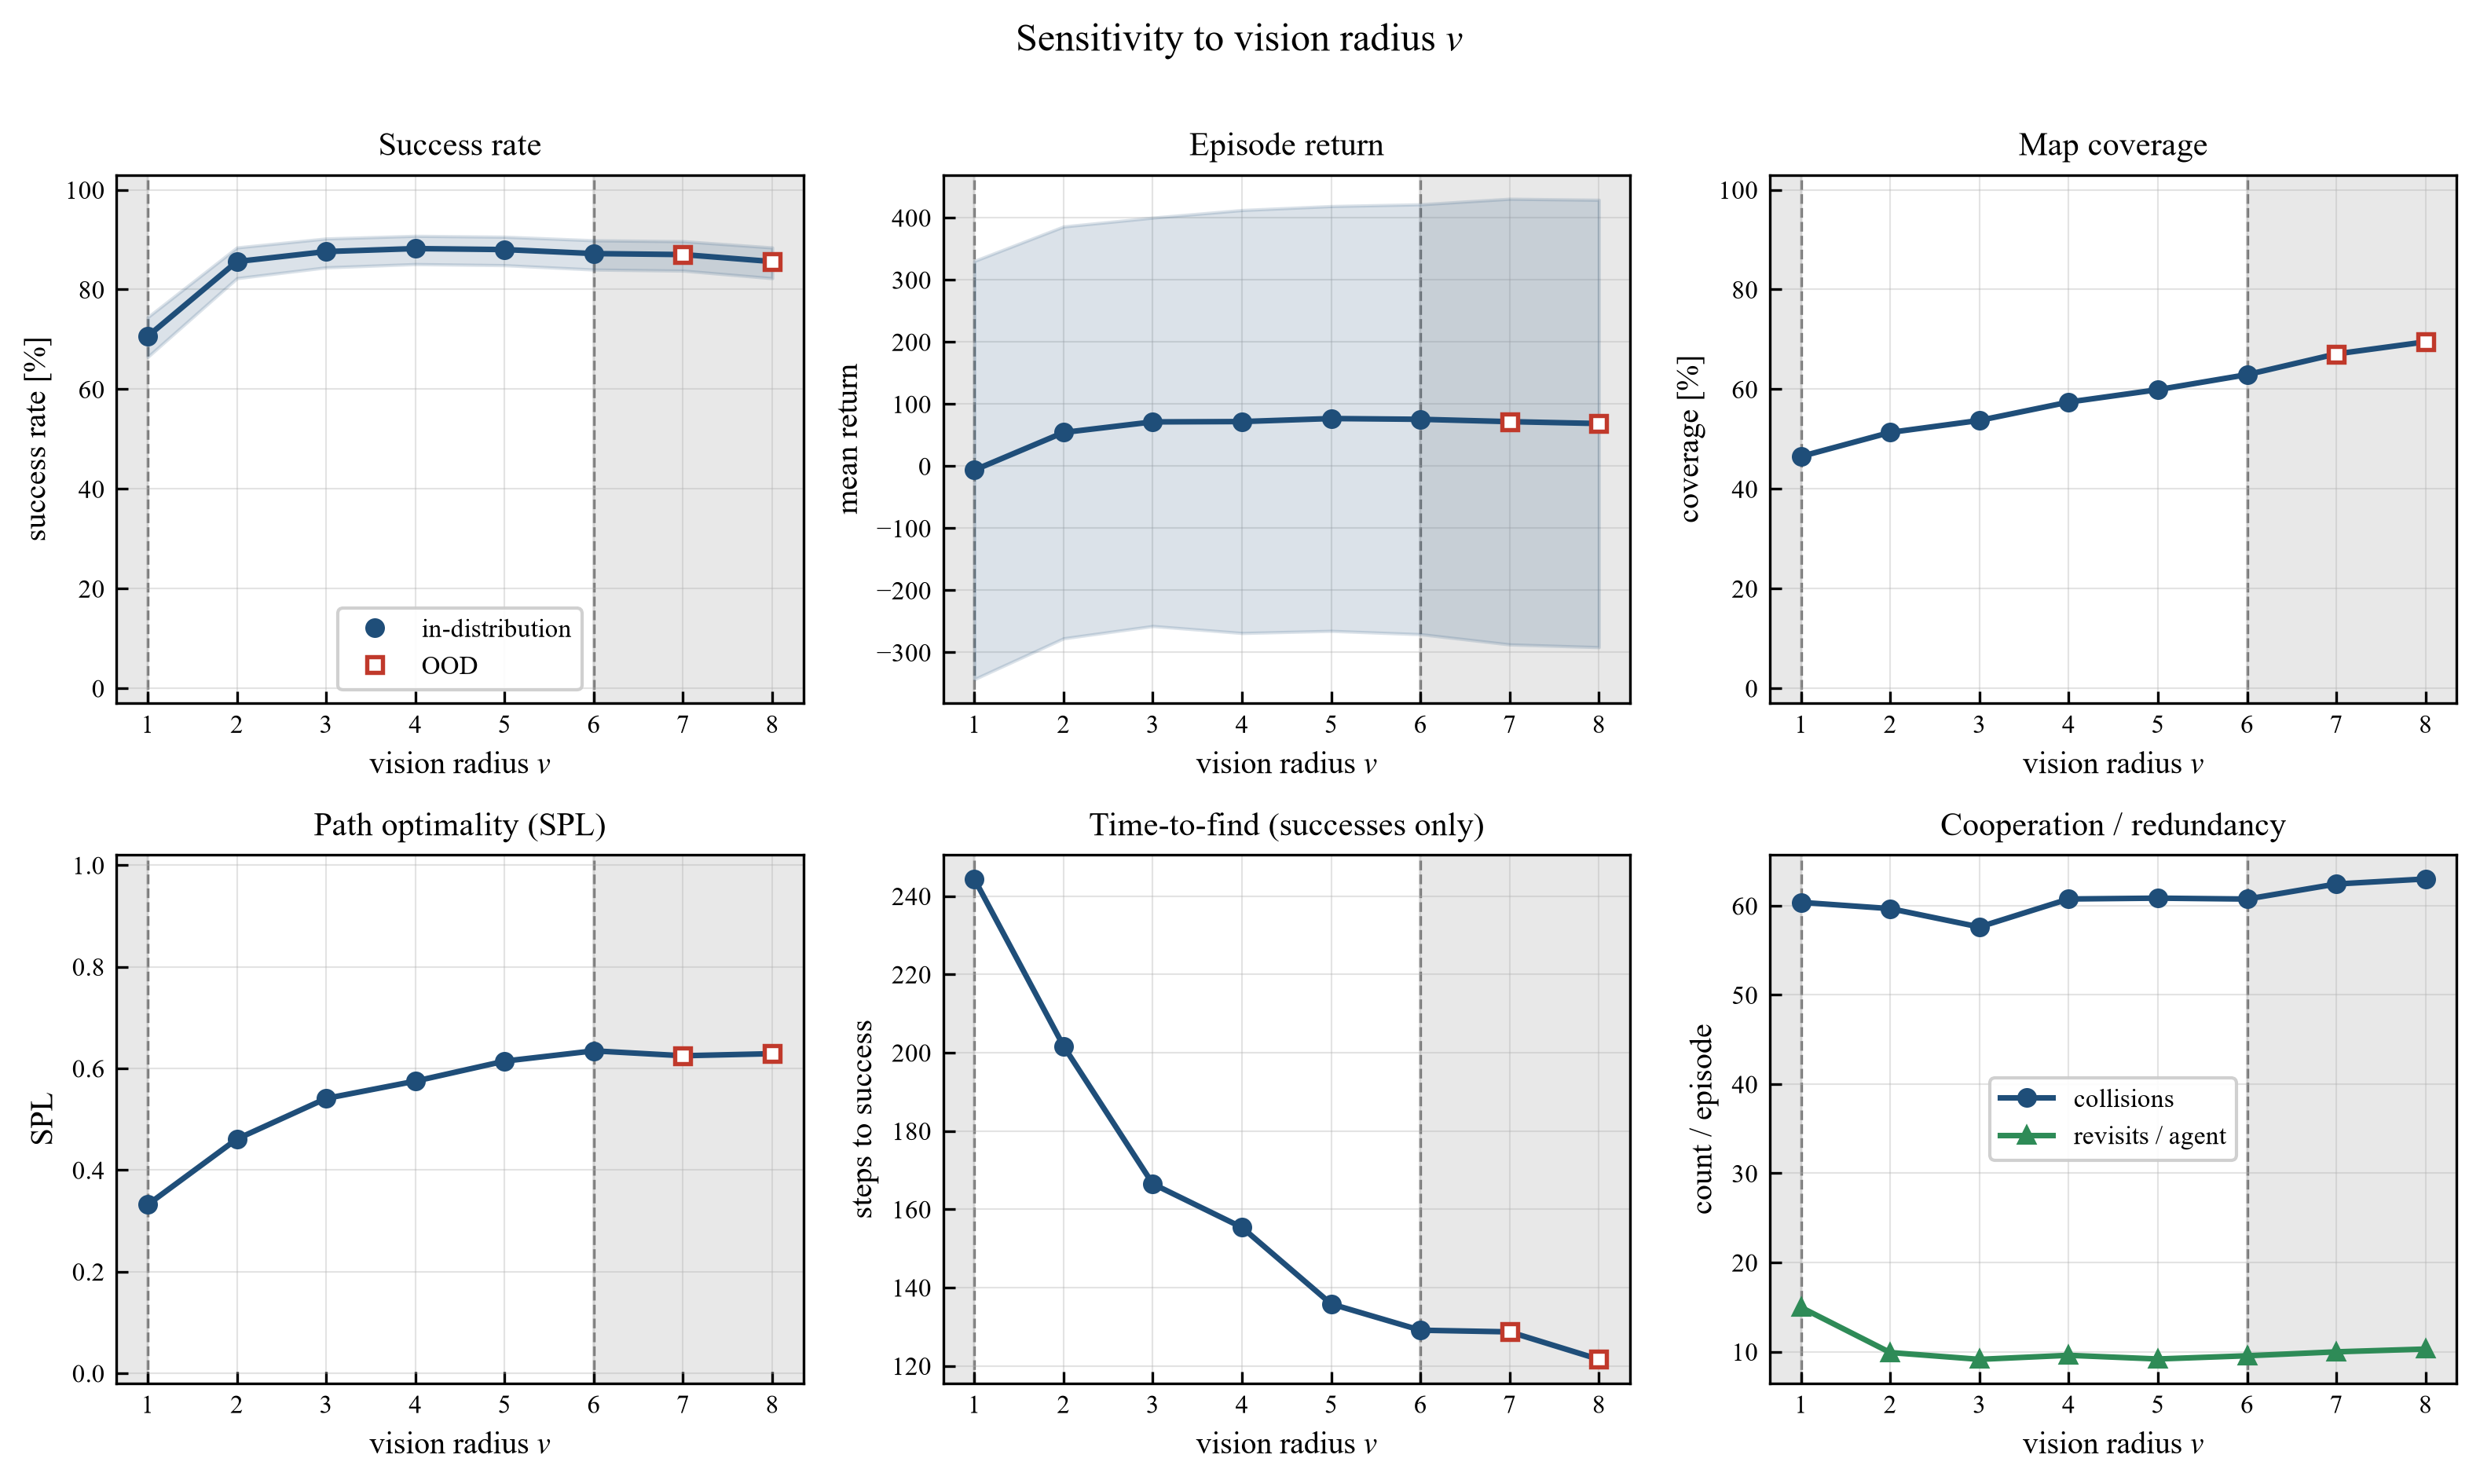
\includegraphics[width=\textwidth]{fig_vision.png}
\caption{Sensitivity to vision radius $\rvis$. Coverage rises monotonically
with sight (top right), but success saturates around $\rvis = 3\text{--}4$:
past a point the bottleneck is deciding where to go, not seeing farther. The
OOD radii $\rvis = 7, 8$ (shaded) degrade only slightly.}
\label{fig:app-vision}
\end{figure}

\begin{figure}[h]
\centering
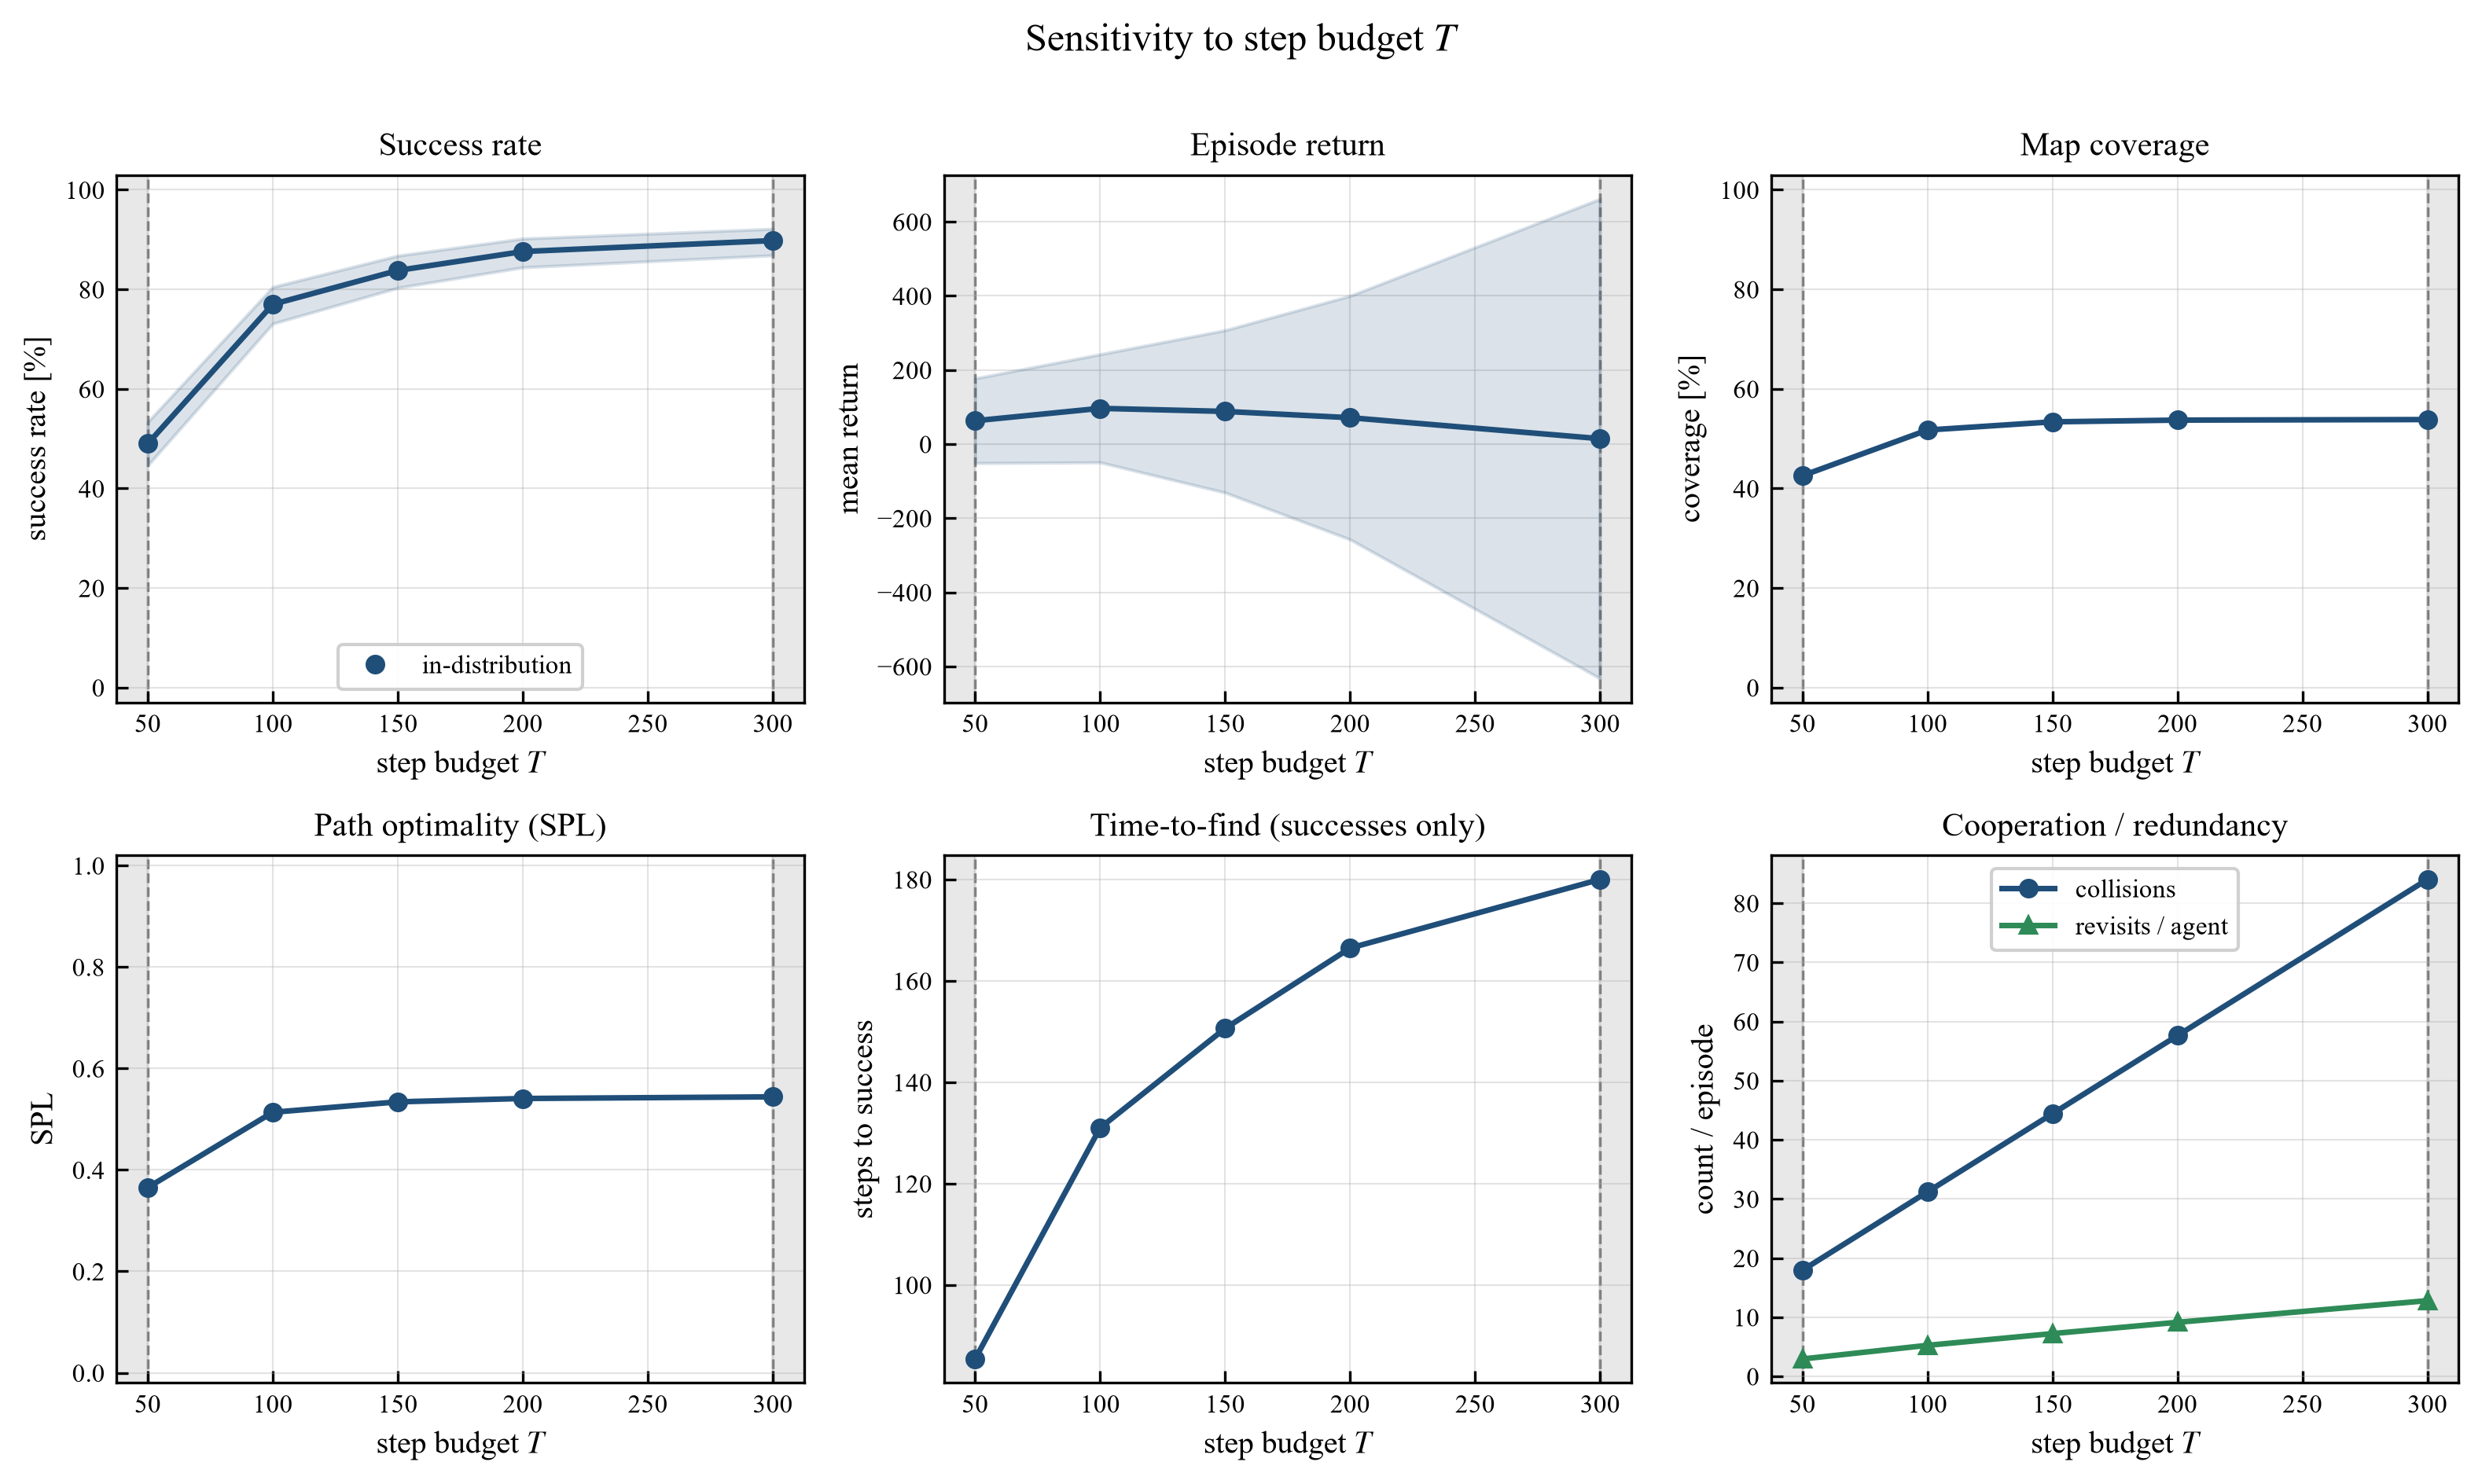
\includegraphics[width=\textwidth]{fig_max_steps.png}
\caption{Sensitivity to the step budget $T$. Success rises with diminishing
returns as the budget grows; a larger budget only rescues episodes that were
already close to succeeding. No OOD region is defined for this axis (the
budget is not a randomized factor).}
\label{fig:app-maxsteps}
\end{figure}

\begin{figure}[t]
\centering
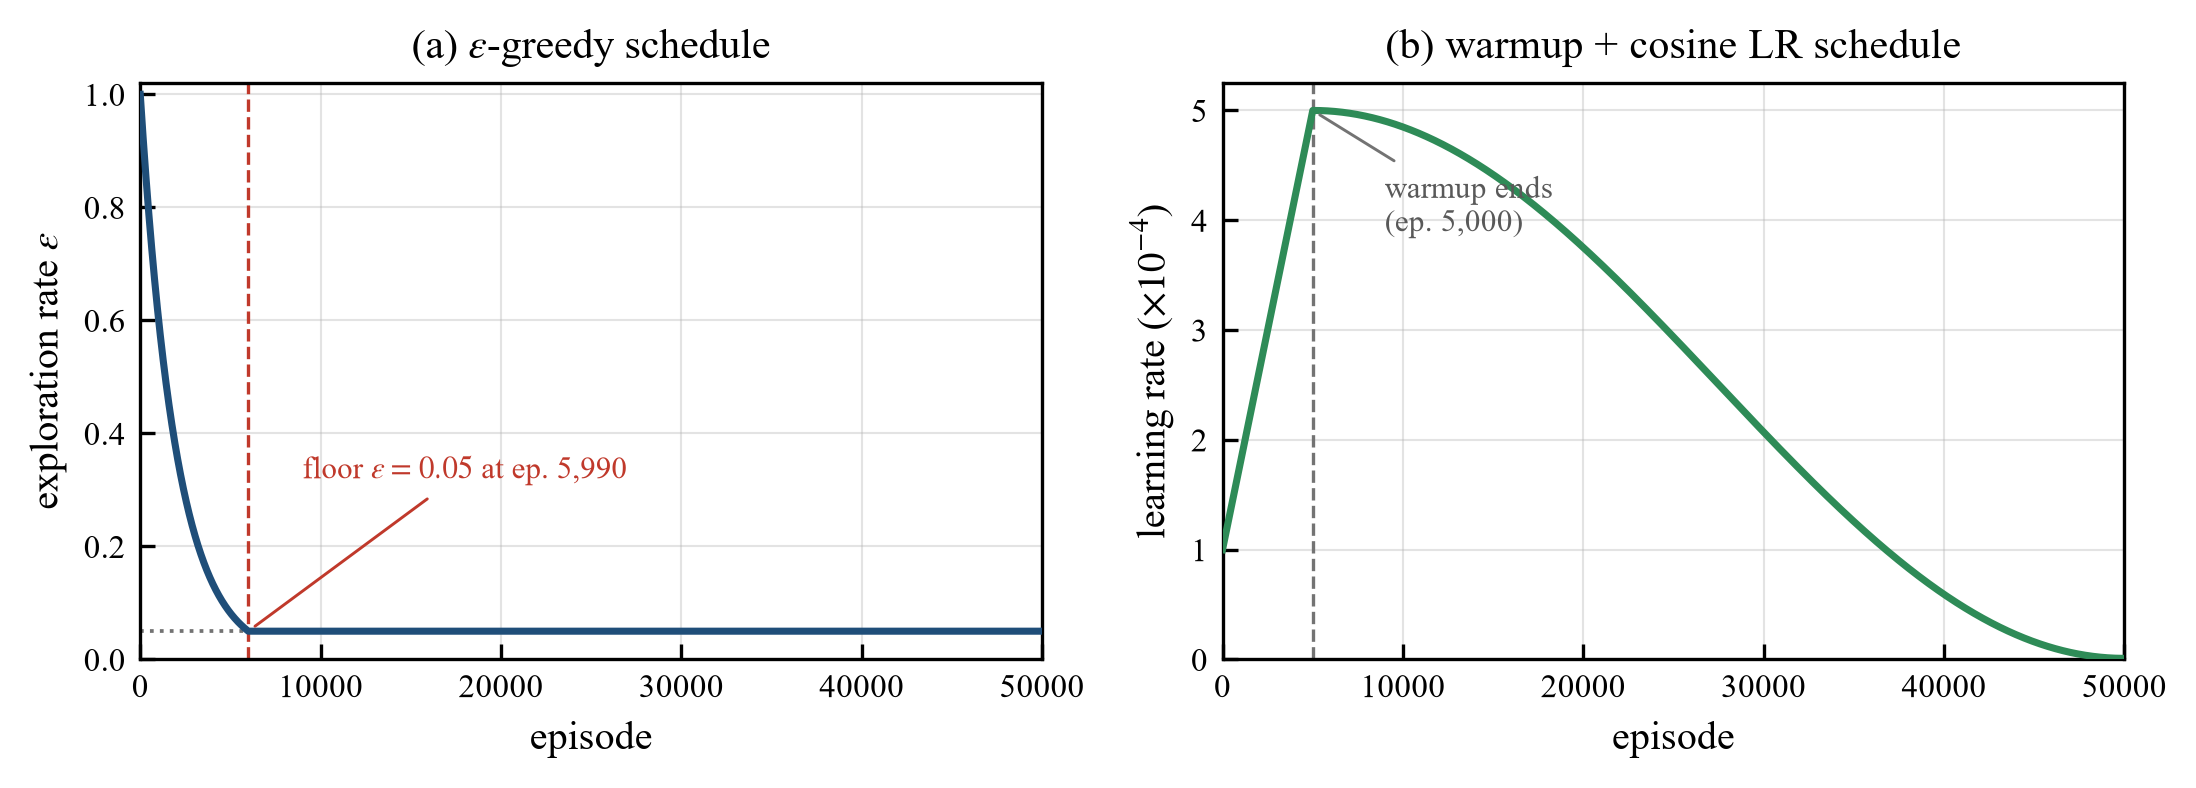
\includegraphics[width=0.92\textwidth]{fig_schedules.png}
\caption{The two per-episode schedules of the final $50{,}000$-episode run.
\emph{(a)} $\varepsilon$ decays multiplicatively to its $0.05$ floor at episode
$5{,}990$; \emph{(b)} the learning rate warms up over the first $10\%$ of
episodes to $5\times10^{-4}$, then anneals cosine-wise to $10^{-6}$. The two are
deliberately out of phase: exploration has essentially finished annealing while
the learning rate is still near its peak, so the bulk of the high-learning-rate
budget is spent on a near-greedy --- and therefore task-relevant --- state
distribution.}
\label{fig:schedules}
\end{figure}

\begin{figure}[t]
\centering
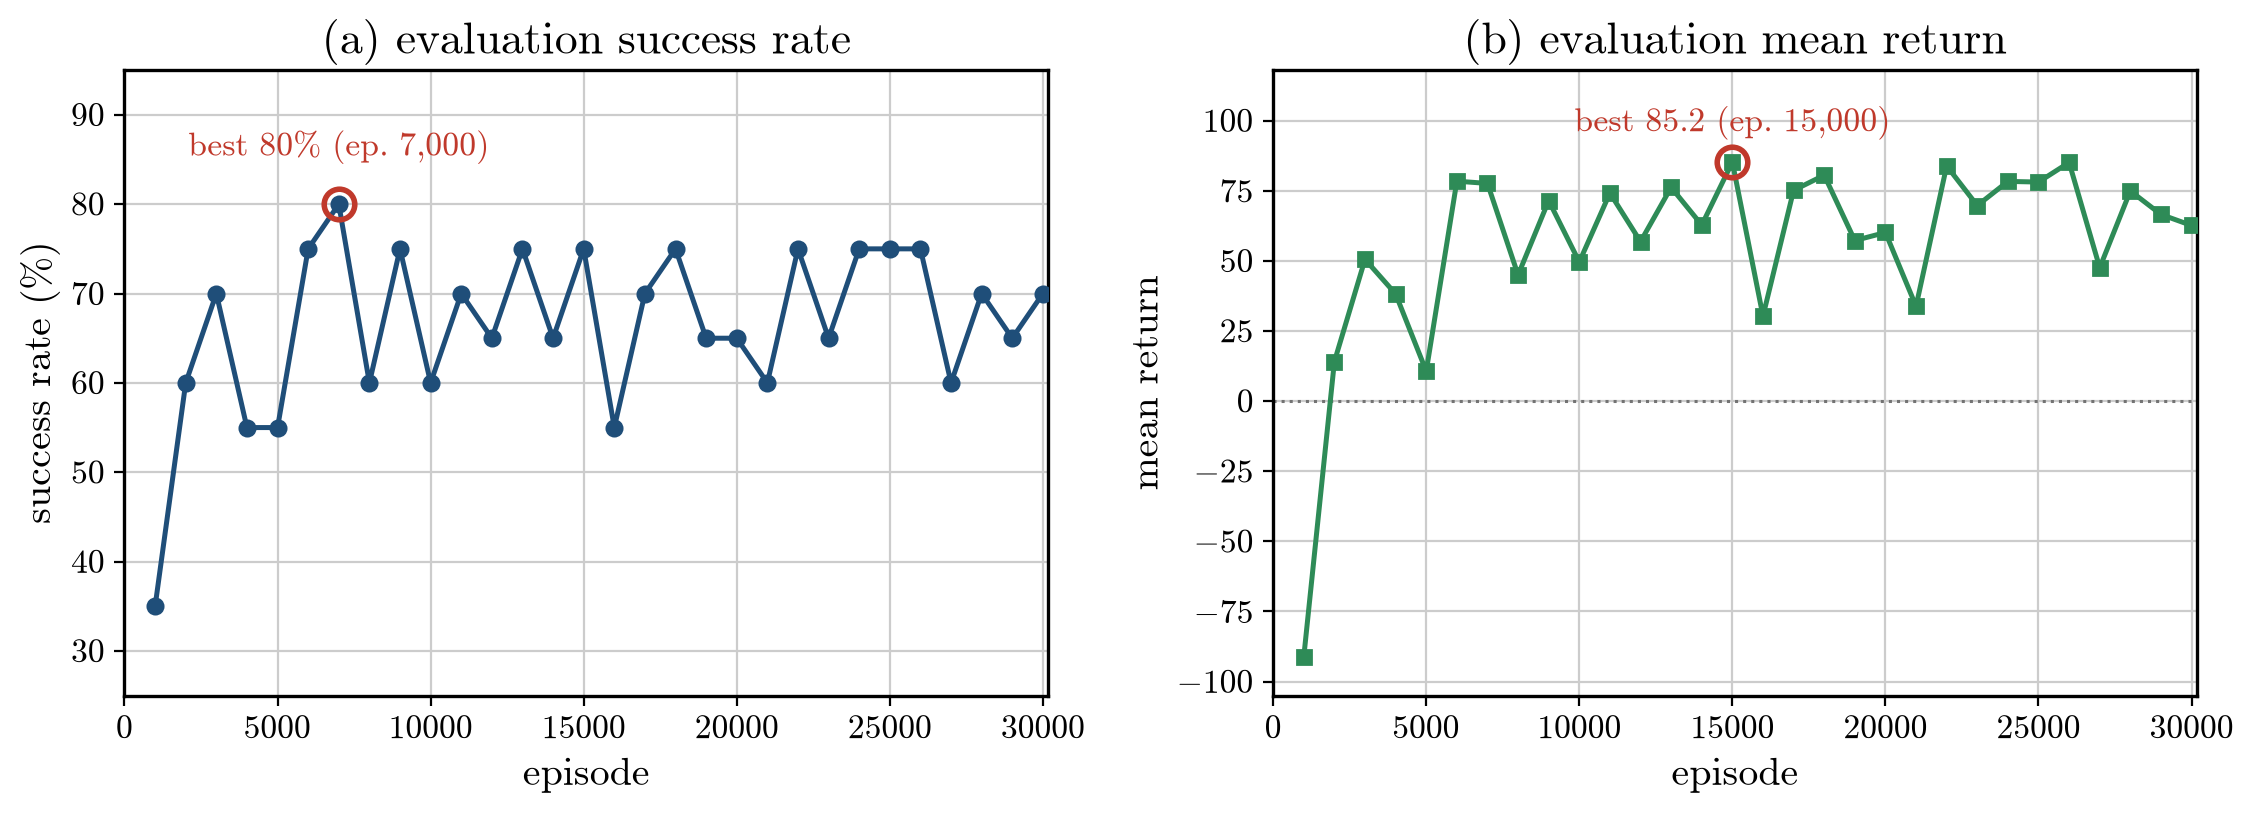
\includegraphics[width=0.86\textwidth]{fig_training_eval.png}
\caption{In-training greedy evaluation of the same run, executed every $1{,}000$
episodes on the fixed bank of $20$ seeded instances that drives checkpoint
selection; \emph{(a)} success rate and \emph{(b)} mean return, best values
circled. These levels are not comparable with those of
Section~\ref{sec:experiments}: this bank samples the \emph{full} randomization
ranges --- solo drones, $\rvis{=}1$, faults active --- whereas
Section~\ref{sec:experiments} measures at the reference operating point. The
$5$-point sawtooth in \emph{(a)} is the quantization of a $20$-instance bank,
which is the noise the strict-improvement selection rule is designed not to
chase. Both panels flatten by around episode $7{,}000$.}
\label{fig:training-eval}
\end{figure}

\begin{figure}[t]
\centering
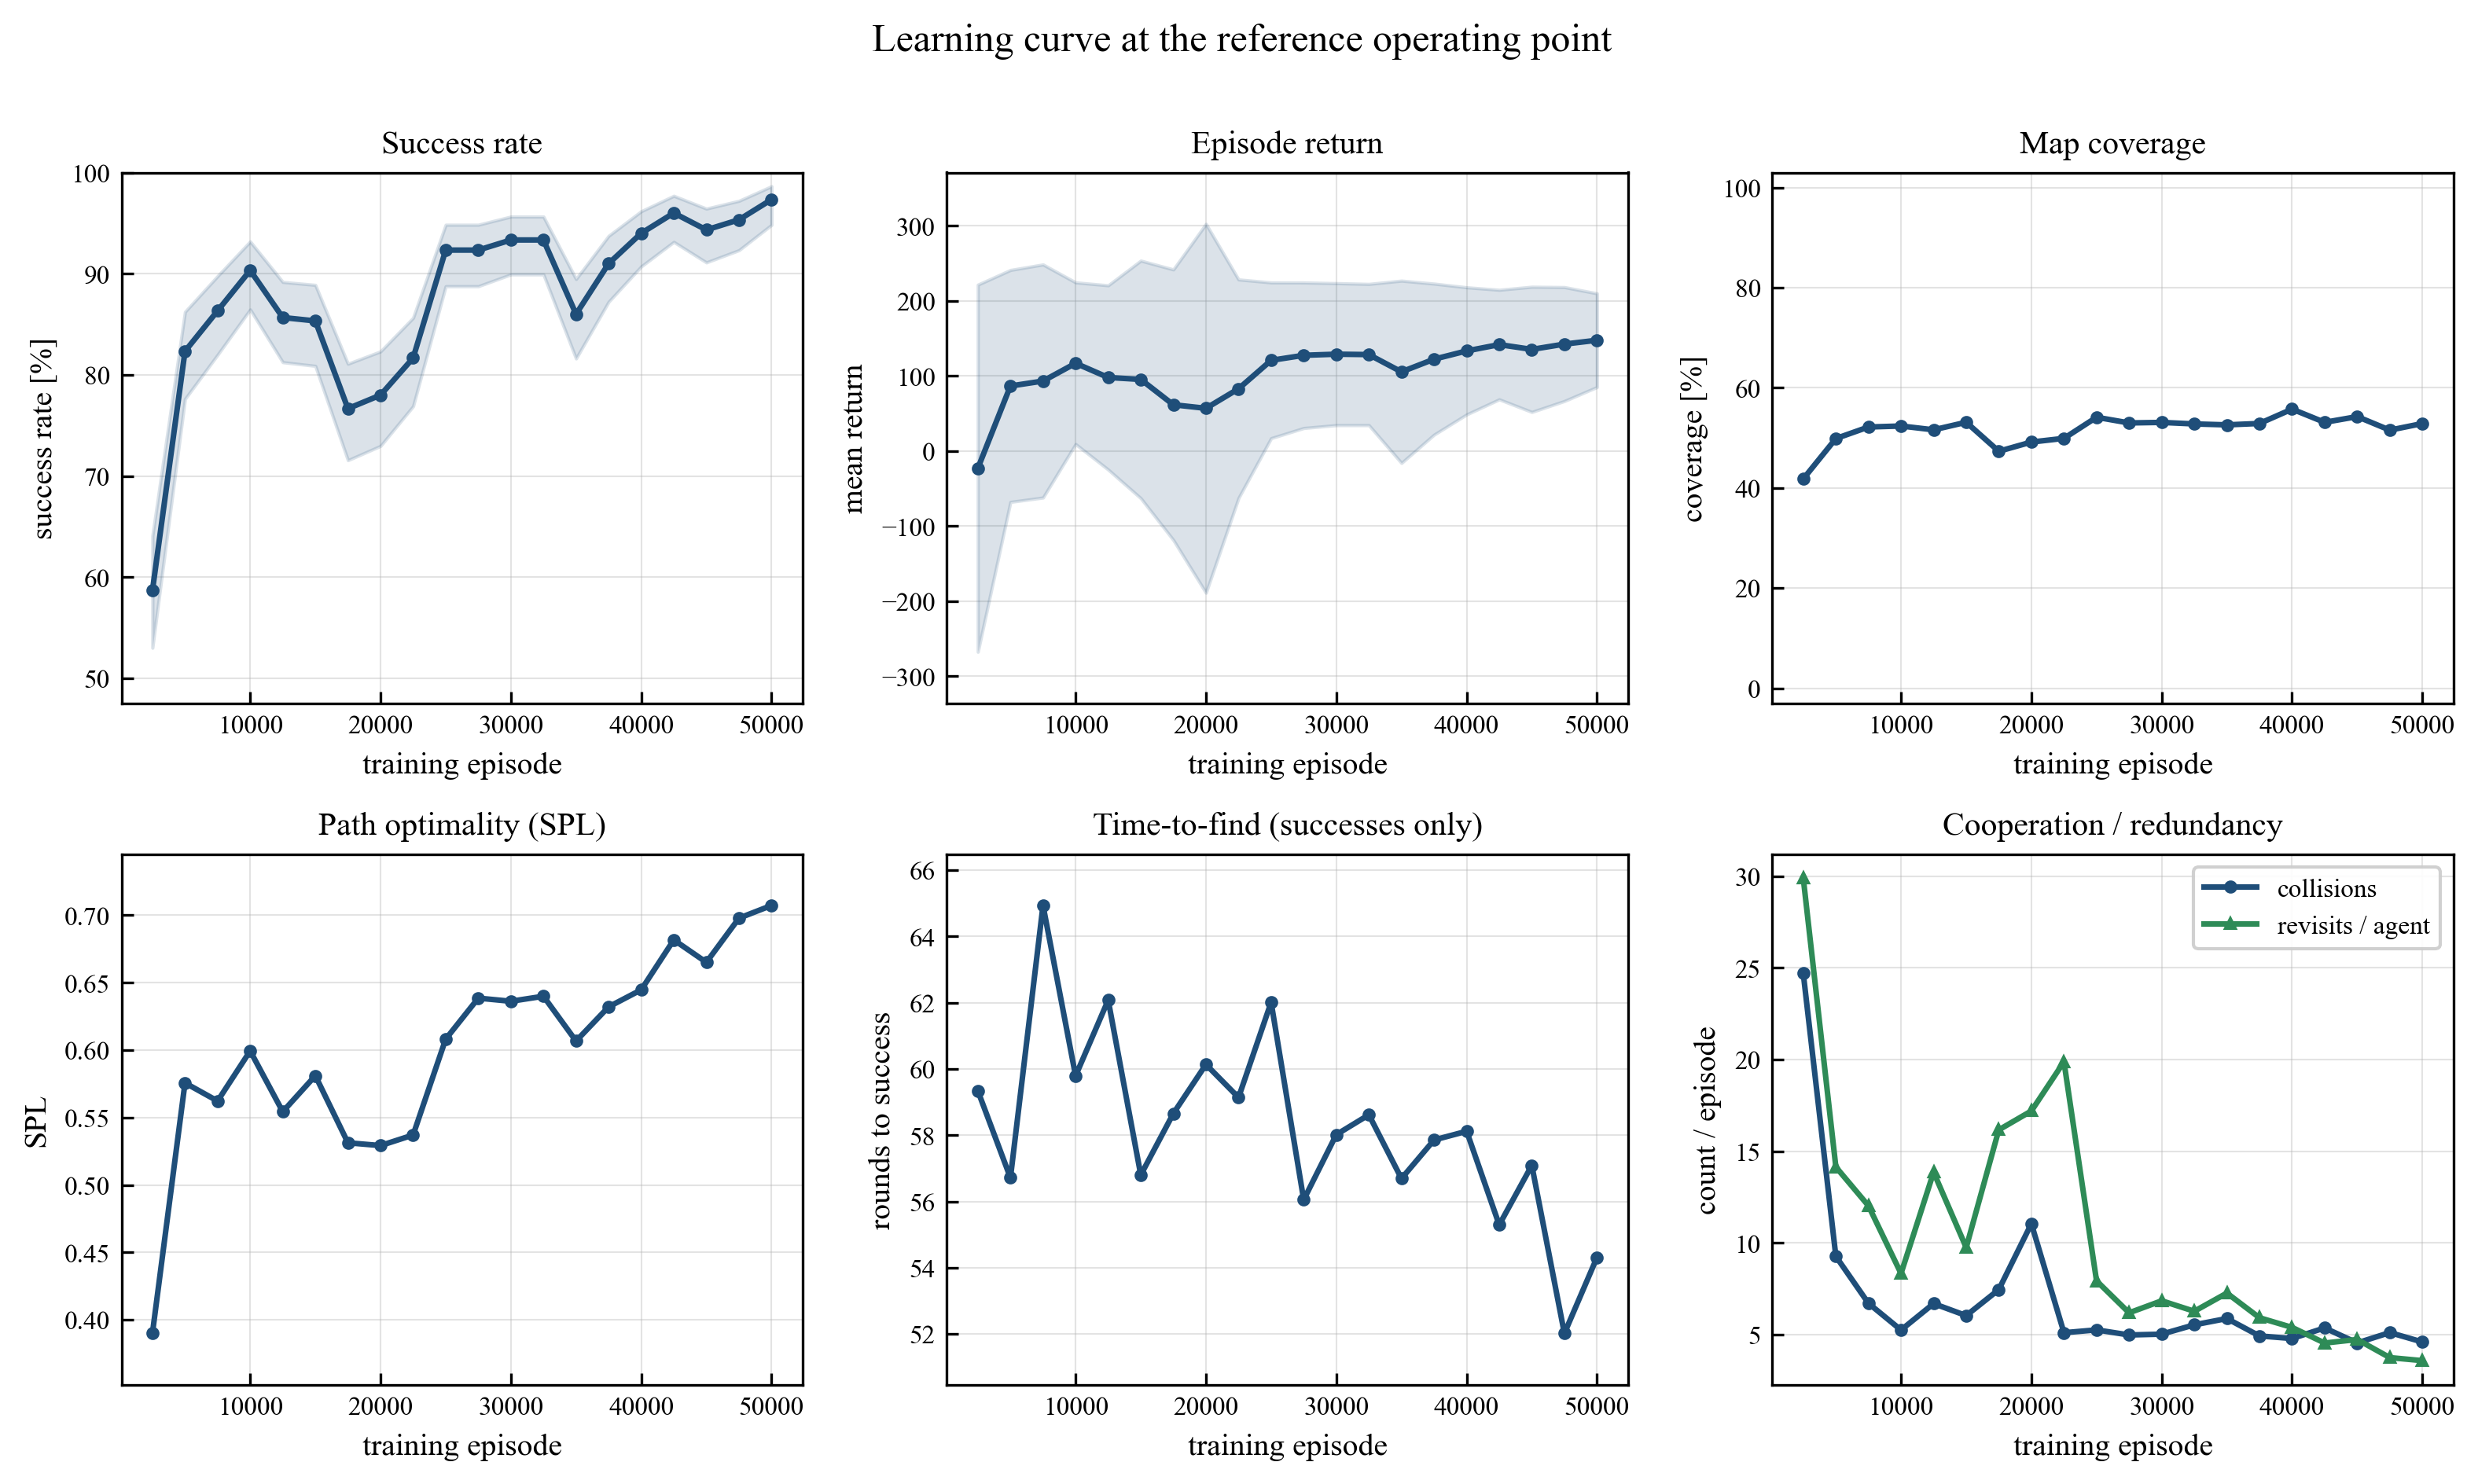
\includegraphics[width=0.86\textwidth]{fig_epoch.png}
\caption{Learning curve: every periodic checkpoint of the final run,
evaluated greedily at the reference operating point ($300$ seeds). Success
plateaus near $85\%$ while SPL keeps improving, indicating late refinement of
path quality rather than of find rate.}
\label{fig:epoch}
\end{figure}


% The bibliography is set one size down and on a tightened inter-entry skip:
% 62 entries at body size and natbib's default \bibsep run to five pages, and
% the course caps the report at 50.
{\small
\setlength{\bibsep}{0.15ex plus 0.1ex}
\bibliographystyle{plainnat}
\bibliography{references}
}

\end{document}
